% Options for packages loaded elsewhere
\PassOptionsToPackage{unicode}{hyperref}
\PassOptionsToPackage{hyphens}{url}
%
\documentclass[
]{book}
\usepackage{amsmath,amssymb}
\usepackage{lmodern}
\usepackage{iftex}
\ifPDFTeX
  \usepackage[T1]{fontenc}
  \usepackage[utf8]{inputenc}
  \usepackage{textcomp} % provide euro and other symbols
\else % if luatex or xetex
  \usepackage{unicode-math}
  \defaultfontfeatures{Scale=MatchLowercase}
  \defaultfontfeatures[\rmfamily]{Ligatures=TeX,Scale=1}
\fi
% Use upquote if available, for straight quotes in verbatim environments
\IfFileExists{upquote.sty}{\usepackage{upquote}}{}
\IfFileExists{microtype.sty}{% use microtype if available
  \usepackage[]{microtype}
  \UseMicrotypeSet[protrusion]{basicmath} % disable protrusion for tt fonts
}{}
\makeatletter
\@ifundefined{KOMAClassName}{% if non-KOMA class
  \IfFileExists{parskip.sty}{%
    \usepackage{parskip}
  }{% else
    \setlength{\parindent}{0pt}
    \setlength{\parskip}{6pt plus 2pt minus 1pt}}
}{% if KOMA class
  \KOMAoptions{parskip=half}}
\makeatother
\usepackage{xcolor}
\IfFileExists{xurl.sty}{\usepackage{xurl}}{} % add URL line breaks if available
\IfFileExists{bookmark.sty}{\usepackage{bookmark}}{\usepackage{hyperref}}
\hypersetup{
  pdftitle={Assessing Urban Quality at the Parcel Level},
  pdfauthor={Carole Voulgaris and Elizabeth Christoforetti},
  hidelinks,
  pdfcreator={LaTeX via pandoc}}
\urlstyle{same} % disable monospaced font for URLs
\usepackage{longtable,booktabs,array}
\usepackage{calc} % for calculating minipage widths
% Correct order of tables after \paragraph or \subparagraph
\usepackage{etoolbox}
\makeatletter
\patchcmd\longtable{\par}{\if@noskipsec\mbox{}\fi\par}{}{}
\makeatother
% Allow footnotes in longtable head/foot
\IfFileExists{footnotehyper.sty}{\usepackage{footnotehyper}}{\usepackage{footnote}}
\makesavenoteenv{longtable}
\usepackage{graphicx}
\makeatletter
\def\maxwidth{\ifdim\Gin@nat@width>\linewidth\linewidth\else\Gin@nat@width\fi}
\def\maxheight{\ifdim\Gin@nat@height>\textheight\textheight\else\Gin@nat@height\fi}
\makeatother
% Scale images if necessary, so that they will not overflow the page
% margins by default, and it is still possible to overwrite the defaults
% using explicit options in \includegraphics[width, height, ...]{}
\setkeys{Gin}{width=\maxwidth,height=\maxheight,keepaspectratio}
% Set default figure placement to htbp
\makeatletter
\def\fps@figure{htbp}
\makeatother
\setlength{\emergencystretch}{3em} % prevent overfull lines
\providecommand{\tightlist}{%
  \setlength{\itemsep}{0pt}\setlength{\parskip}{0pt}}
\setcounter{secnumdepth}{5}
\usepackage{booktabs}
\usepackage{booktabs}
\usepackage{longtable}
\usepackage{array}
\usepackage{multirow}
\usepackage{wrapfig}
\usepackage{float}
\usepackage{colortbl}
\usepackage{pdflscape}
\usepackage{tabu}
\usepackage{threeparttable}
\usepackage{threeparttablex}
\usepackage[normalem]{ulem}
\usepackage{makecell}
\usepackage{xcolor}
\usepackage{caption}
\usepackage{graphicx}
\usepackage{siunitx}
\usepackage{hhline}
\usepackage{calc}
\usepackage{tabularx}
\usepackage{adjustbox}
\usepackage{hyperref}
\ifLuaTeX
  \usepackage{selnolig}  % disable illegal ligatures
\fi
\usepackage[]{natbib}
\bibliographystyle{plainnat}

\title{Assessing Urban Quality at the Parcel Level}
\author{Carole Voulgaris and Elizabeth Christoforetti}
\date{}

\begin{document}
\maketitle

{
\setcounter{tocdepth}{1}
\tableofcontents
}
\hypertarget{introduction}{%
\chapter{Introduction}\label{introduction}}

Elizabeth will write 2,000 words or so about the motivations and vision for
this project.

\hypertarget{report-organization}{%
\section{Report organization}\label{report-organization}}

The remainder of this report proceeds as follows. Chapter 2 discusses related
work that we and others have done on the topic of evaluating urban quality
and the challenges of highly-disaggregated spatial data. In Chapter 3, we
describe a set of workshops we conducted with a diverse set of experts on
urban development to identify values associated with urban quality. We go on
to propose a method for evaluating urban quality at the parcel level using
readily available data for Allegheny County, Pennsylvania in Chapter 4, and
summarize the results of that analysis in Chapter 5. In Chapter 6, we discuss
the alignment of the values suggested in our workshops with the outcomes
of our quantitative analysis. Chapter 7 concludes the report with our key
takeaways and potential directions for future work.

\hypertarget{related-work}{%
\chapter{Related work}\label{related-work}}

\hypertarget{neighborhood-classification}{%
\section{Neighborhood classification}\label{neighborhood-classification}}

There is a large body of literature that seeks to apply quantitative methods to
describe or classify urban environments. In 2011, Urban Geography released a
special issue devoted to neighborhood classification approaches, including a
review of neighborhood classification work that had been done to date \citep{reibel2011classification};
a study identifying five distinct neighborhood types in Cleveland and
demonstrating how locations transition among types \citep{mikelbank2011neighborhood};
a method for identifying ethnic neighborhoods \citep{logan2011identifying}; and an
analysis of New Urban developments that classifies them by how well they meet the
ambitions of the New Urbanism movement \citep{trudeau2011suburbs}. A common approach to
classifying neigborhoods has been to employ factor analysis (principal
component analysis) to reduce a large number
of variables into a smaller set of factors (or principal components), followed by
cluster analysis to group neighborhoods sharing similar characteristics \citep{voulgaris_synergistic_2016, chow_differentiating_1998, li_neighborhood_2009, shay_automobiles_2007, song_quantitative_2007, song_how_2008, vicino_typology_2011}.
Although the purpose of neighborhood classification studies is to develop a set
of categorical neighborhood types, the initial factor analysis step yields a set
of indices that can be used as continuous variables describing various dimensions
of neighborhood characteristics.

\hypertarget{quantification-of-sprawl}{%
\section{Quantification of sprawl}\label{quantification-of-sprawl}}

In general, neighborhood classification studies have differentiated between
neighborhoods with a more urban character and those with a more suburban
character. Indeed this is often the explicit purpose of such analyses. A
related body of work has specifically sought to quanitify sprawl. \citet{hamidi2015measuring}
offers a helpful review of the early work on this topic, noting that early studies
emphasized density as a measure of sprawl and that some used satellite imagery
to incorporate parameters like fragmentation and fractal dimension. \citet{ewing_measuring_2002}
have developed a widely-cited measure of sprawl using principal component analysis
to develop indices for four separate dimensions of sprawl (density, land-use diversity,
centering, and street accessibility) and averaging them (with equal weights) to generate
a single overall sprawl index. \citet{hamidi2015measuring} later repeated this method with
updated data and have published a dataset of county-level and tract-level values
for the resulting sprawl index.

\hypertarget{conceptualizing-urban-quality-at-the-site-level}{%
\section{Conceptualizing urban quality at the site level}\label{conceptualizing-urban-quality-at-the-site-level}}

\hypertarget{expert-perspectives}{%
\chapter{Expert Perspectives}\label{expert-perspectives}}

Summarize the workshops.

\hypertarget{quantitative-methods}{%
\chapter{Quantitative Methods}\label{quantitative-methods}}

How might results of quantitative approach to evaluating urban quality at the
parcel level align with the values identified in the workshops described in
Chapter 3? In this chapter, we propose one such approach, using
readily-available parcel-level data for Allegheny County, Pennsylvania.

\hypertarget{data}{%
\section{Data}\label{data}}

We obtained data on property addresses, land uses, assessed values (for both
land and buildings), and sale prices
from \citet{allegheny_county_office_of_property_assessments_allegheny_2022}, which
includes information on 582,116 properties in Allegheny County.

We also obtained latitude and longitude coordinates for each property from a
geocoder file provided by \citet{western_pennsylvania_regional_data_center_geocoders_2021}.
Over 99.5 percent of properties included in the assessment dataset are included
in the geocoder file. Properties without geocoded locations are excluded from
our analysis.

Potential development sites were identified as those

\begin{enumerate}
\def\labelenumi{\arabic{enumi}.}
\item
  classified as ``residential'' (residential properties with one to
  four housing units) or ``commercial'' (which includes mixed-use developments
  and residential properties with more than four housing units), and
\item
  with a land use description in one of 59 possible categories\footnote{One site (3008
    Phillip Dr in Clairton) is missing a land use description in the assessment data.
    We checked this address on Zillow to determine that this is a single-family home
    and classified it as such in our data.}. The most common of these are listed Table \ref{tab:list-site-uses}.\footnote{The land use descriptions that were
    classified as potential development sites but are not listed in Table
    \ref{tab:list-site-uses}, which combine to represent less than one percent of all sites
    are ``RIGHTOF WAY - RESIDENTIAL'', ``CONDOMINIUM UNIT'', ``DWG USED AS OFFICE'',
    ``APART:20-39 UNITS'', ``CONDO GARAGE UNITS'', ``COMMON AREA'', ``CONDO DEVELOPMENTAL
    LAND'', ``CONDEMNED/BOARDED-UP'', ``CONDOMINIUM OFFICE BUILDING'', ``INDEPENDENT LIVING
    (SENIORS)'', ``DWG USED AS RETAIL'', ``OTHER COMMERCIAL'', ``MOBILE HOMES/TRAILER PKS'',
    ``RIGHT OF WAY - COMMERCIAL'', ``GROUP HOME'', ``TOTAL/MAJOR FIRE DAMAGE - COMM'',
    ``OTHER COMMERCIAL HOUSING'', ``TOTAL/MAJOR FIRE DAMAGE'', ``COMM APRTM CONDOS 5-19
    UNITS'', ``MUNICIPAL URBAN RENEWAL'', ``COMMERCIAL LAND'', ``CAMPGROUNDS'', ``COMMON AREA
    OR GREENBELT'', ``CHARITABLE EXEMPTION/HOS/HOMES'', ``INCOME PRODUCING PARKING LOT'',
    ``DWG APT CONVERSION'', ``\textgreater10 ACRES VACANT'', ``MINOR FIRE DAMAGE'', ``COMM APRTM CONDOS
    20-39 UNITS'', ``COMMERCIAL/UTILITY'',
    ``H.O.A RECREATIONS AREA'', ``COMM APRTM CONDOS 40+ UNITS'', ``MINOR FIRE DAMAGE - COMM'',
    ``OTHER'', ``OTHER RESIDENTIAL STRUCTURE'', ``OWNED BY METRO HOUSING AU'', ``RESIDENTIAL VACANT
    LAND'', ``HUD PROJ \#221'', and ``VACANT LAND 0-9 ACRES''}.
\end{enumerate}

\begin{table}

\caption{\label{tab:list-site-uses}Most common land uses categorized as potential sites}
\centering
\begin{tabu} to \linewidth {>{\raggedright}X>{\raggedleft}X>{\raggedleft}X>{\raggedleft}X}
\toprule
USEDESC & Number of potential sites & Percent of potential sites & Cumulative percent of potential sites\\
\midrule
SINGLE FAMILY & 370,513 & 73.2 & 73.2\\
VACANT LAND & 62,672 & 12.4 & 85.5\\
TWO FAMILY & 17,293 & 3.4 & 89.0\\
TOWNHOUSE & 14,670 & 2.9 & 91.8\\
ROWHOUSE & 11,082 & 2.2 & 94.0\\
\addlinespace
VACANT COMMERCIAL LAND & 5,817 & 1.1 & 95.2\\
THREE FAMILY & 3,968 & 0.8 & 96.0\\
RES AUX BUILDING (NO HOUSE) & 3,601 & 0.7 & 96.7\\
RETL/APT'S OVER & 3,354 & 0.7 & 97.3\\
COMM AUX BUILDING & 2,825 & 0.6 & 97.9\\
\addlinespace
APART: 5-19 UNITS & 2,771 & 0.5 & 98.4\\
FOUR FAMILY & 2,058 & 0.4 & 98.9\\
BUILDERS LOT & 1,230 & 0.2 & 99.1\\
PARKING GARAGE/LOTS & 891 & 0.2 & 99.3\\
OFFICE/APARTMENTS OVER & 854 & 0.2 & 99.4\\
\addlinespace
MOBILE HOME & 666 & 0.1 & 99.6\\
APART:40+ UNITS & 529 & 0.1 & 99.7\\
DWG USED AS OFFICE & 440 & 0.1 & 99.8\\
APART:20-39 UNITS & 400 & 0.1 & 99.8\\
CONDEMNED/BOARDED-UP & 132 & 0.0 & 99.9\\
\bottomrule
\end{tabu}
\end{table}

Potential building sites were further filtered to exclude those with missing data
on the most recent sale (about one percent of all sites).\footnote{Four sites had sales
  prices listed that were unreasonably high. 3039 Liberty Avenue in Pittsburgh is
  listed as having sold for \$511,945,000 on August 30, 2021. Zillow lists this
  property as having sold on that date for \$511,945
  (\url{https://www.zillow.com/homedetails/3039-W-Liberty-Ave-Pittsburgh-PA-15216/2070262638_zpid/}, accessed 5/4/2022),
  so the value was corrected for what appears to have been a typo. 220 Hyeholde Dr
  in Coraopolis is listed as having sold for \$28,100,000 in 1967. This may also
  be a typo, and it also does not seem to be the most recent sale. Zillow lists
  this home as having sold for \$350,000 in 2004
  (\url{https://www.zillow.com/homes/220-hyeholde-dr,-Coraopolis,-PA_rb/11552817_zpid/},
  accessed 5/4/2022), so the data was corrected to add that as the most recent sale.
  Two other sites were identified as having unreasonably high sales values: 1339
  Arlington Avenue in Pittsburgh is a three-bedroom single-family home that is
  listed as having sold for \$57,010,813 in 1976 and a 0.06-acre vacant lot with
  tax ID 0165G00270000000 is listed as having sold for \$24,920,232 in 1936. The
  sales data for these sites were treated as missing.}

The focus of this analysis is on potential development sites rather than on
properties. Some properties in the assessor dataset are condominums where
multiple properties share a single parcel of land. We aggregated these to the
site level by identifying all properties with an assessed building value
greater than zero, a land value of zero, and a land use description that did
not indicate the land was vacant. If multiple such properties share an address,
we classified all properties at that address as a condominium and aggregated
them to the parcel level. This led to a final sample of 506,405 sites.

\hypertarget{tax-assessment-data}{%
\subsection{Tax assessment data}\label{tax-assessment-data}}

Three variables (total assessed fair market value, assessed fair market
value of the building, and lot area) were taken directly from the county
tax assessment data for use in our analysis. We also included the most
recent listed sales price, adjusted for inflation.

To aggregate properties identified as condominiums to the site level, we summed
the total values for lot area, assessed land value, assessed building value, and
inflation-adjusted sale price. We log-transformed these four variables prior to
including them in our analysis. Their distributions are shown in
Figure \ref{fig:assessor-hist}.

\begin{figure}
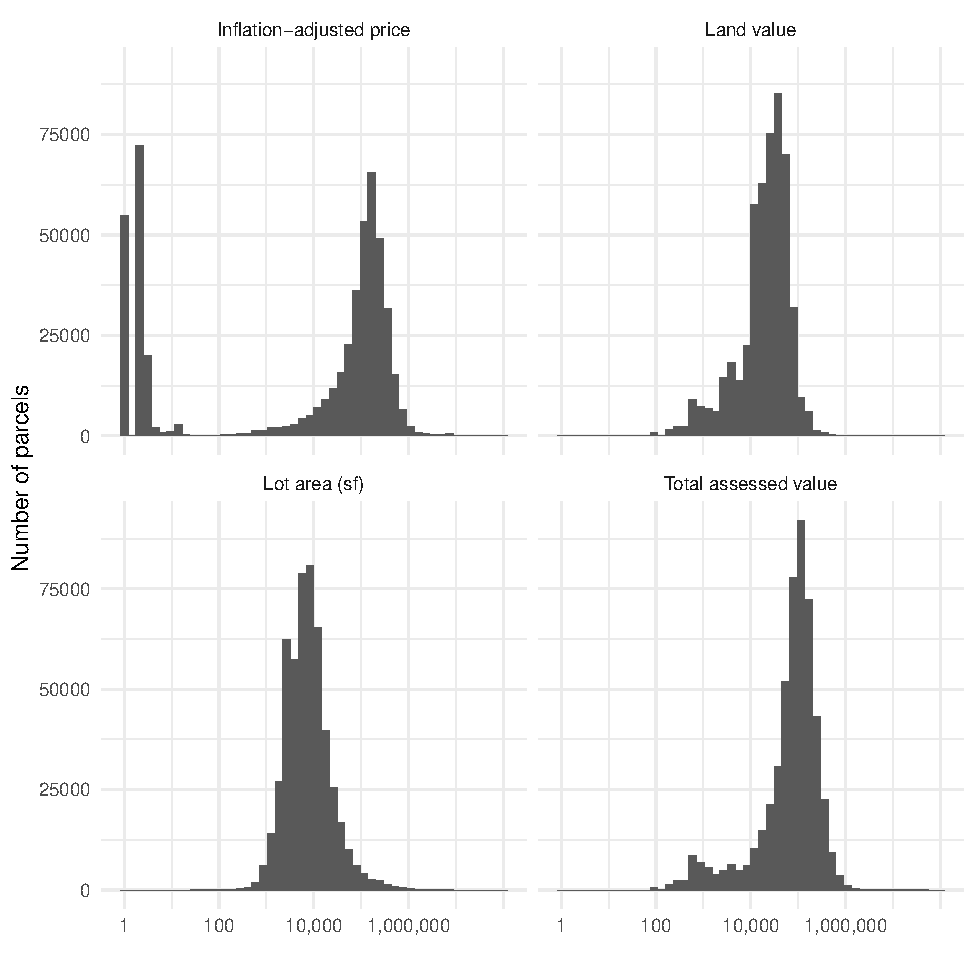
\includegraphics[width=1\linewidth]{_main_files/figure-latex/assessor-hist-1} \caption{Distribution of variables from tax assessor database}\label{fig:assessor-hist}
\end{figure}

\hypertarget{accessibilty-data}{%
\subsection{Accessibilty data}\label{accessibilty-data}}

Accessibilty was calculated from each of the 518,032 sites in our sample to
each of several location types described below.

\hypertarget{destination-parcels}{%
\subsubsection{Destination parcels}\label{destination-parcels}}

We used land use codes from the county assessor parcel data to identify
\emph{destination parcels} that residents might value access to. The most common
land use codes of identified destination parcels are listed in Table \ref{tab:dest-uses}.

\begin{table}

\caption{\label{tab:dest-uses}Land uses identified as potential destinations}
\centering
\begin{tabu} to \linewidth {>{\raggedright}X>{\raggedleft}X>{\raggedleft}X>{\raggedleft}X}
\toprule
USEDESC & Number of identified destinations & Percent of identified destinations & Cumulative percent of identified destinations\\
\midrule
MUNICIPAL GOVERNMENT & 10,376 & 29.88 & 29.88\\
CHURCHES, PUBLIC WORSHIP & 1,946 & 5.60 & 35.49\\
COMMERCIAL GARAGE & 1,735 & 5.00 & 40.48\\
OFFICE - 1-2 STORIES & 1,649 & 4.75 & 45.23\\
SMALL DETACHED RET(UNDER 10000) & 1,646 & 4.74 & 49.97\\
\addlinespace
OFFICE/WAREHOUSE & 1,386 & 3.99 & 53.96\\
COUNTY GOVERNMENT & 1,287 & 3.71 & 57.67\\
WAREHOUSE & 1,252 & 3.61 & 61.27\\
OWNED BY BOARD OF EDUCATION & 1,086 & 3.13 & 64.40\\
TOWNSHIP GOVERNMENT & 855 & 2.46 & 66.86\\
\addlinespace
LIVESTOCK O/T D \& P-CAUV & 805 & 2.32 & 69.18\\
LIGHT MANUFACTURING & 799 & 2.30 & 71.48\\
PUBLIC PARK & 710 & 2.04 & 73.53\\
RESTAURANT, CAFET AND/OR BAR & 697 & 2.01 & 75.54\\
GENERAL FARM & 607 & 1.75 & 77.28\\
\addlinespace
OWNED BY COLLEGE/UNIV/ACADEMY & 458 & 1.32 & 78.60\\
MEDICAL CLINICS/OFFICES & 445 & 1.28 & 79.88\\
RETL/OFF OVER & 442 & 1.27 & 81.16\\
OFFICE-ELEVATOR -3 + STORIES & 412 & 1.19 & 82.34\\
LODGE HALL/AMUSEMENT PARK & 386 & 1.11 & 83.46\\
\bottomrule
\end{tabu}
\end{table}

\hypertarget{job-locations}{%
\subsubsection{Job locations}\label{job-locations}}

We identified \emph{job locations} based on data from a Longitudinal
Employer-Household Dynamics (LEHD) dataset published by the United States Census
Bureau \citep{united_states_census_bureau_lehd_2021}. The LEHD dataset provides the
total number of jobs in each census block in the United States, based on
employment tax records. The location of each job was defined as the centroid of
the block in which it was located. We downloaded job location data for
Pennsylvania and filtered it to include locations in the Pittsburgh metropolitan
area (Allegheny, Armstrong, Beaver, Butler, Fayette, Washington, and
Westmoreland counties).

In addition to calculating the accessibility to jobs of all categories, we also
calculated accessibility to several subsets of jobs. We disaggregated jobs by
earnings, reasoning that the usefulness of a job might vary depending on how
well it matches a workers skills or wage expectations. \emph{High-paying job locations}
are a subset of job locations where the worker earns more than \$3333 per month.
\emph{Low-paying job locations} are those where the worker earns \$1250 per month or less.

We also disaggregated jobs based on employment industry, based on the North
American Industry Classification System (NAICS), reasoning that the presence of
jobs particular industries might represent a shopping or recreation destination.
\emph{Retail job locations} are a subset of job locations in NAICS sector 44-45
(retail trade); \emph{Entertainment job locations} are those in NAICS sector 71
(arts, entertainment, and recreation); and \emph{Hospitality job locations} are
those in NAICS sector 72 (accommodation and food services).

Finally, we identified three location types that correspond with common non-work
trips: schools, grocery stores, and parks. \emph{Grocery store locations} were
identified as vendors participating in the Supplemental Nutrition Program for
Women, Infants, and Children (WIC). WIC vendor locations and \emph{school locations}
were obtained from the Allegheny County GIS portal
\citep{allegheny_county_office_of_information_technology_allegheny_2018, allegheny_county_office_of_information_technology_allegheny_2020}.
\emph{Park locations} were taken from the Pennsylvania Geospatial Data Clearinghouse
\citep{pennsylvania_department_of_conservation_and_natural_resources_pennsylvania_2015}.
Park locations were downloaded for Pennsylvania and filtered to Allegheny county.

We used the r5r package in the R programming language \citep{pereira_r5r_2021} to
calculate accessibility each destination type described above,
for each of four transportation modes (walking, cycling, driving, and transit).
The r5r package calculates accessibility as the weighted total number of
destinations reachable by a given mode, where destinations are weighted
according to a decay function, such that destinations that can be reached within
less time are assigned greater weight. We used a logistic decay function, as
illustrated in \ref{fig:show-decay-func}. For motorized modes, the decay
function had a mean (inflection) of 40 minutes and a standard deviation of 10
minutes. For non-motorized modes, the decay function had a mean of 20 minutes
and a standard deviation of 5 minutes.

\begin{figure}

{\centering 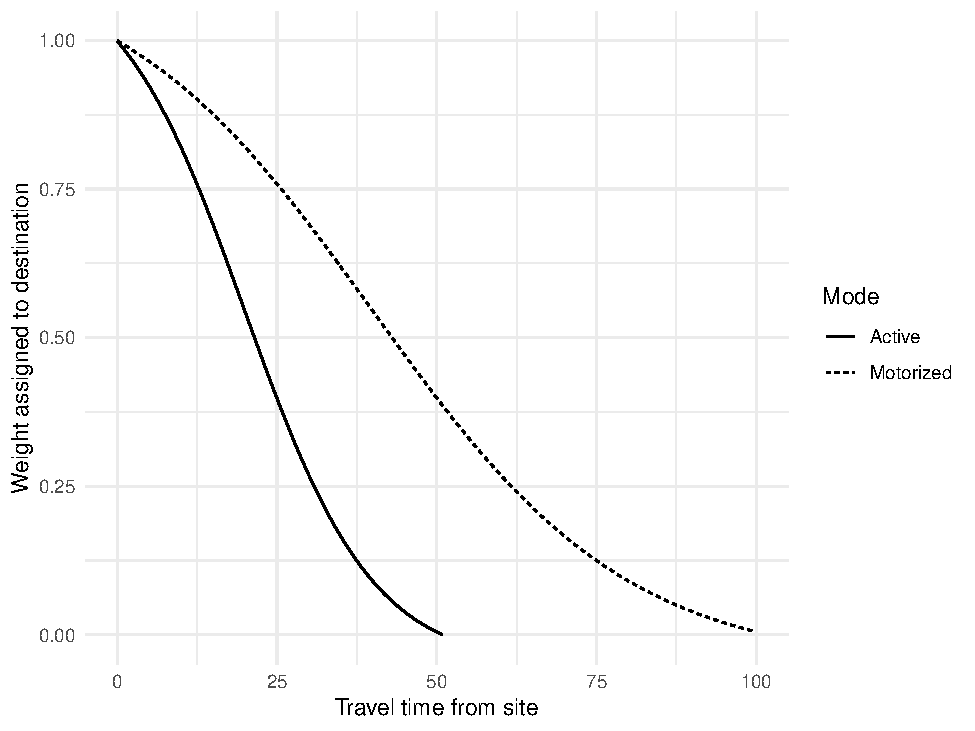
\includegraphics[width=0.8\linewidth]{_main_files/figure-latex/show-decay-func-1} 

}

\caption{Decay functions for accessibility calculations}\label{fig:show-decay-func}
\end{figure}

Calculating accessibility metrics for a combination of four transportation
modes and ten destination types yields 40 different accessibility variables. Figure \ref{fig:show-decay-func}
illustrates the distributions of each of these variables.

\begin{figure}

{\centering 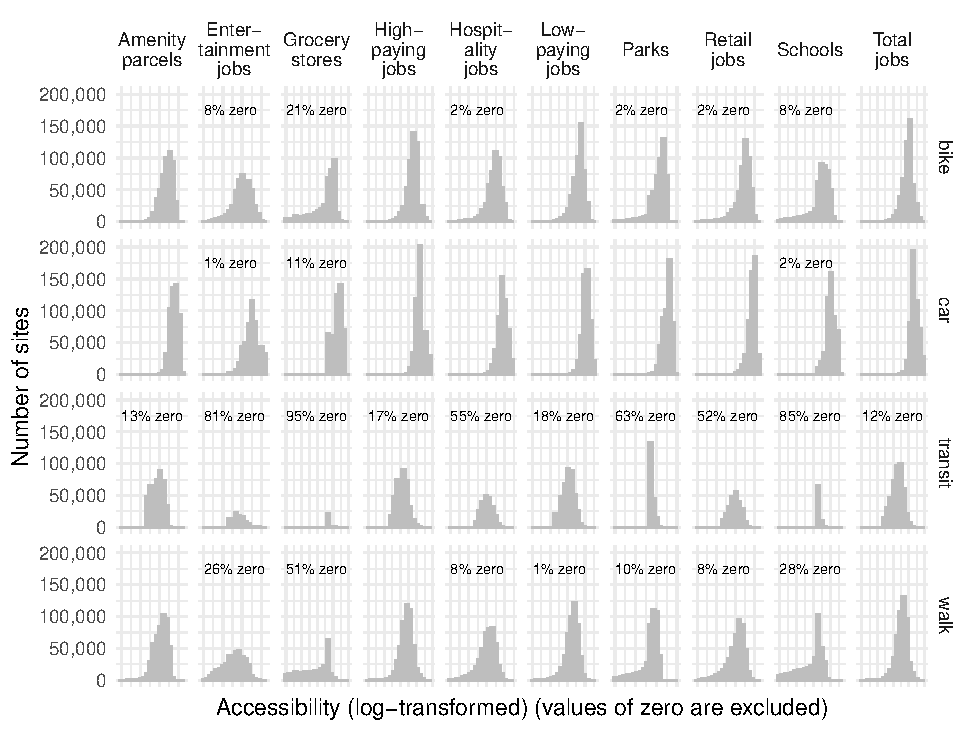
\includegraphics[width=1\linewidth]{_main_files/figure-latex/access-dist-1} 

}

\caption{Distributions of accessibility variables}\label{fig:access-dist}
\end{figure}

\hypertarget{disamenity-proximity}{%
\subsection{Disamenity proximity}\label{disamenity-proximity}}

We categorized several land uses in the county assessor data as
disamenities. The land use codes we used to identify disamenities are
listed in \ref{tab:bad-use-list}\footnote{289 properties related to coal mining
  (with land use descriptions of either ``COAL RIGHTS, WORKING INTERESTS'' or
  ``COAL LAND, SURFACE RIGHTS'') are co-located and are treated as a single
  site.}.

\begin{table}

\caption{\label{tab:bad-use-list}Land uses identified as disamenities}
\centering
\begin{tabu} to \linewidth {>{\raggedright}X>{\raggedleft}X>{\raggedleft}X>{\raggedleft}X}
\toprule
USEDESC & Number of identified locations & Percent of identified locations & Cumulative percent of identified locations\\
\midrule
VACANT INDUSTRIAL LAND & 614 & 68.68 & 68.68\\
HEAVY MANUFACTURING & 89 & 9.96 & 78.64\\
FOOD \& DRINK PROCESSING & 40 & 4.47 & 83.11\\
INDUSTRIAL/UTILITY & 39 & 4.36 & 87.47\\
COMMERCIAL TRUCK TERMINAL & 26 & 2.91 & 90.38\\
\addlinespace
RECYCLING/SCRAP YARDS & 23 & 2.57 & 92.95\\
MINES AND QUARRIES & 17 & 1.90 & 94.85\\
P.P. - P.U. - OTHER THAN R.R. & 14 & 1.57 & 96.42\\
INDUSTRIAL TRUCK TERM & 9 & 1.01 & 97.43\\
BULK TRANSFER TERMINAL & 8 & 0.89 & 98.32\\
\addlinespace
INDUSTRIAL LAND & 3 & 0.34 & 98.66\\
POULTRY FARM & 3 & 0.34 & 98.99\\
COAL LAND, SURFACE RIGHTS & 2 & 0.22 & 99.22\\
COAL RIGHTS, WORKING INTERESTS & 2 & 0.22 & 99.44\\
OIL \& GAS RIGHTS WORKING INTEREST & 2 & 0.22 & 99.66\\
\addlinespace
COAL RIGHTS SEP. ROYALTY INTEREST & 1 & 0.11 & 99.78\\
MINERAL LAND & 1 & 0.11 & 99.89\\
OTHER MINERALS & 1 & 0.11 & 100.00\\
\bottomrule
\end{tabu}
\end{table}

We included a disamenity proximity index in our analysis that we calculated
as the logarithm of the average distance from each site to the ten closest
disamenity sites. The distribution of this index is shown in \ref{fig:bad-prox}.

\begin{figure}

{\centering 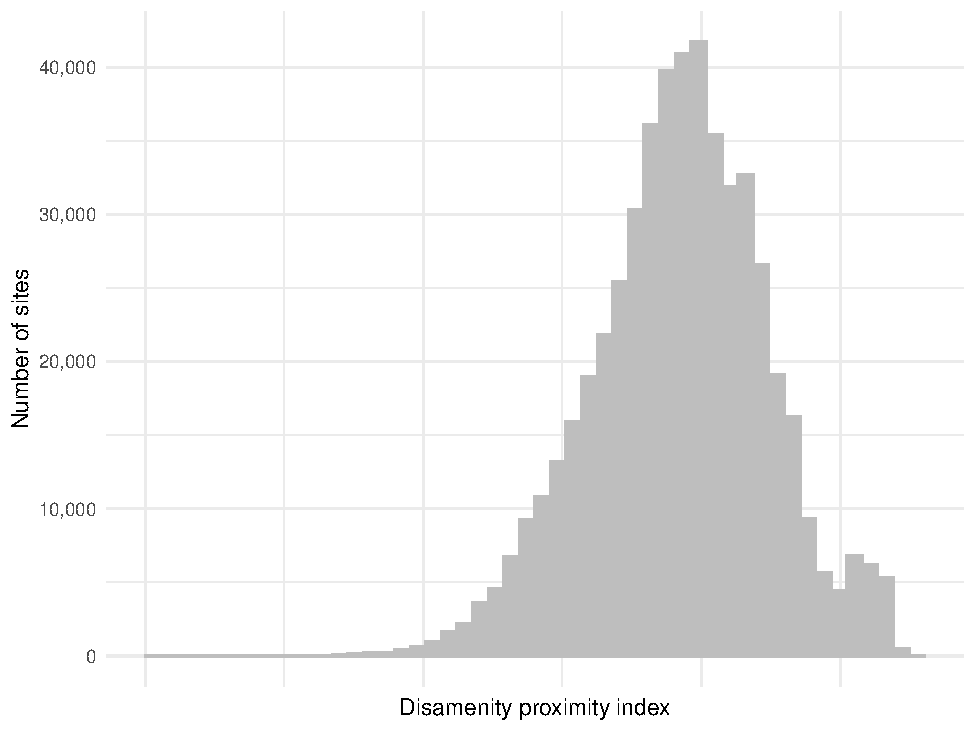
\includegraphics[width=0.8\linewidth]{_main_files/figure-latex/bad-prox-1} 

}

\caption{Distribution of average distance to nearest ten disamenity sites}\label{fig:bad-prox}
\end{figure}

\hypertarget{density}{%
\subsection{Density}\label{density}}

To represent the residential density around each site, we used the sf \citep{sf}, nngeo
\citep{nngeo} and tidycensus \citep{tidycensus} R packages to determine the smallest circular
buffer around each site containing a population of at least two thousand people,
based on the 2020 census. In denser places, a buffer with a smaller radius would
encompass two thousand residents. In more sparsely-populated places, a buffer
containing two thousand residents would be larger. The distribution of radii for
two-thousand-person site buffers is shown in \ref{fig:radii}.

\begin{figure}

{\centering 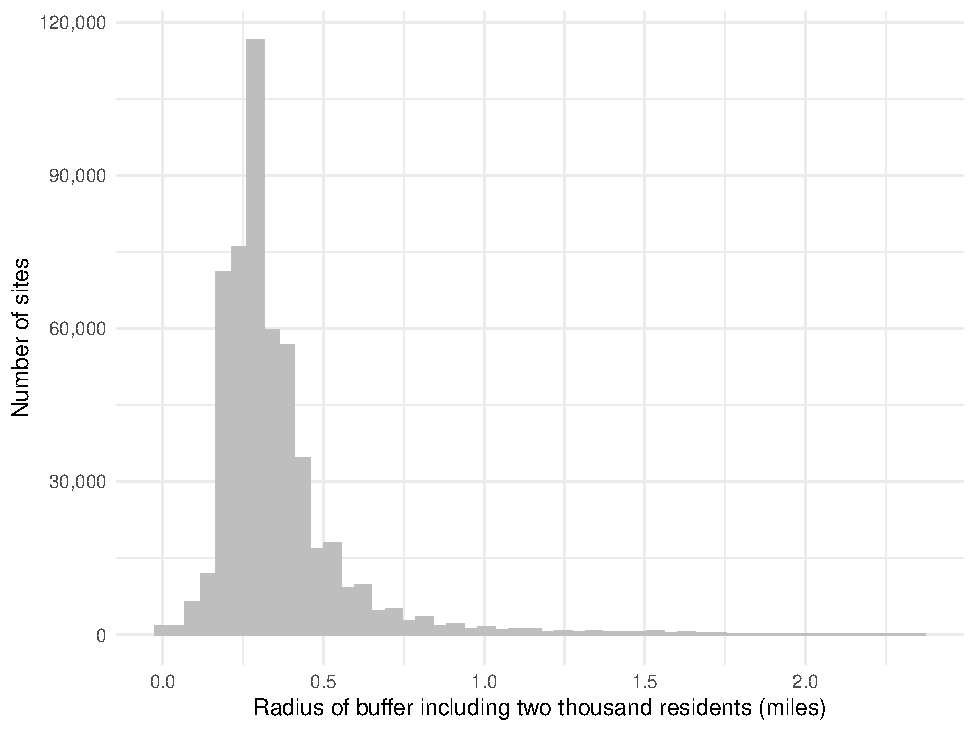
\includegraphics[width=0.8\linewidth]{_main_files/figure-latex/radii-1} 

}

\caption{Histogram of radii of buffer containing 2000 residents}\label{fig:radii}
\end{figure}

\hypertarget{population-diversity}{%
\subsection{Population diversity}\label{population-diversity}}

The two-thousand-resident buffers described above were also used as a basis to
estimate the racial diversity of residents in the immediate vicinity. For each
buffer, we calculated the percentage of residents that who identified in the 2020
census as non-Hispanic white, non-Hispanic Black, and Hispanic. The distributions
of these variables are shown in \ref{fig:divers-hist}.

\begin{figure}

{\centering 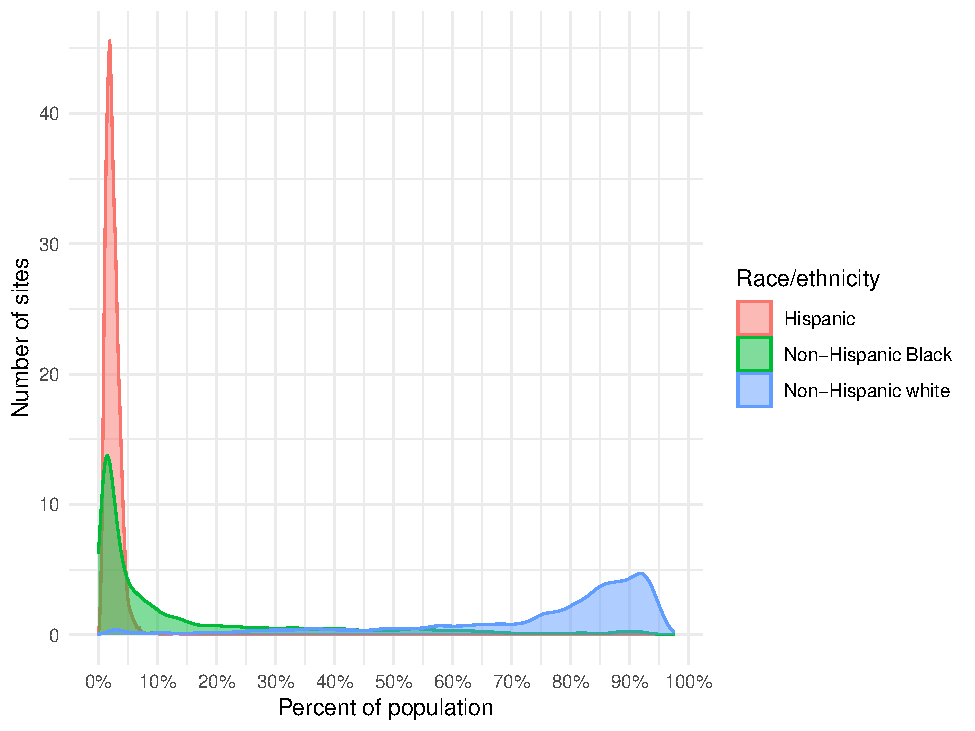
\includegraphics[width=0.8\linewidth]{_main_files/figure-latex/divers-hist-1} 

}

\caption{Distributions of population diversity variables}\label{fig:divers-hist}
\end{figure}

\hypertarget{land-use-diversity}{%
\subsection{Land use diversity}\label{land-use-diversity}}

We also calculated the total number of different land uses within each
two-thousand-resident buffer and used this as a measure of land-use diversity.
\ref{fig:land-divers}.

\begin{figure}

{\centering 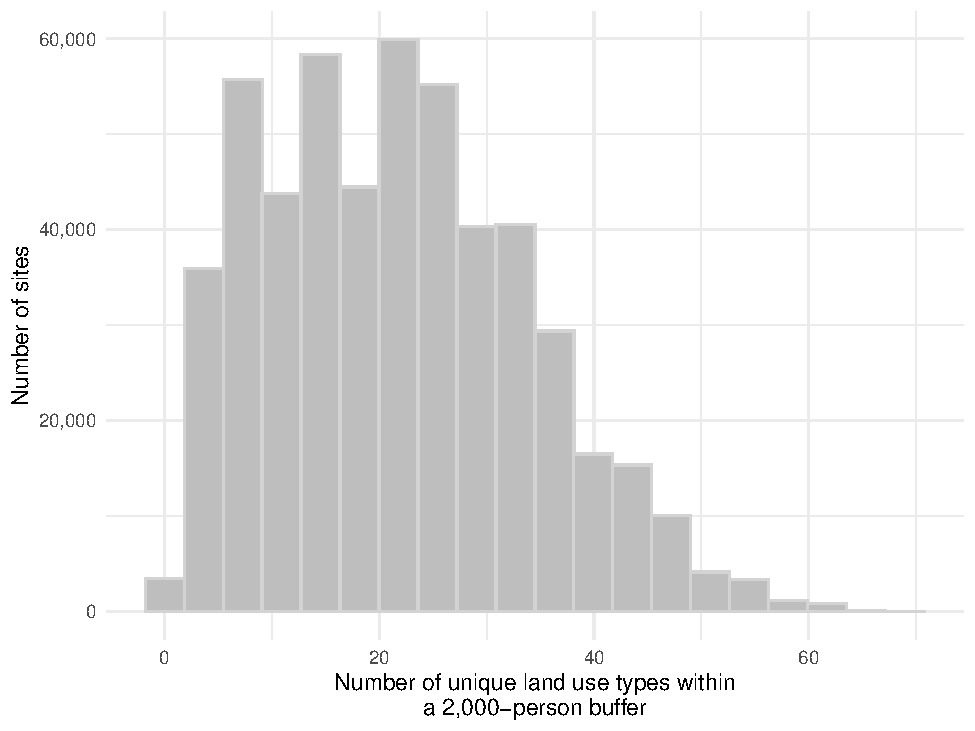
\includegraphics[width=0.8\linewidth]{_main_files/figure-latex/land-divers-1} 

}

\caption{Histogram of land use diversity}\label{fig:land-divers}
\end{figure}

\hypertarget{index-development}{%
\section{Index development}\label{index-development}}

The methods described above yielded a set of fifty parcel-level variables,
forty of which are accessibility metrics, for each of 506,405 parcels. We used
the EFAtools R package \citep{EFAtools} to develop a set of parcel level indices from
these variables using factor analysis. The Kaiser-Meyer-Olkin criterion for the
dataset is 0.9, suggesting a ``marvellous'' case for factor analysis \citep{kaiser1974index}.

We determined the appropriate number of factors based on the Kaiser-Guttman criterion and the Hull method.The Hull method suggests an
optimal number of factors that balances model fit and number of parameters, with a goal
or keeping only major factors. Potential solutions with various number of factors are
plotted on a graph of goodness-of-fit versus degrees of freedom, where the optimal
solution will be on the boundary of a convex hull \citep{lorenzo2011hull}. The Kaiser-Guttmat criterion is a
recommendation to retain as many factors as there are
sample eigenvalues greater than one \citep{guttman1954some}.

We computed factor loadings
using an oblimin rotation. We applied these loadings to calculate a set of index
scores (one for each factor) for each potential development site.

\hypertarget{index-validation}{%
\section{Index validation}\label{index-validation}}

The indices we developed through factor analysis might represent dimensions of
urban quality. If they are valid quality metrics, one might expect them to
be predictive of an activity associated with desirable locations for development.

We hypothesize that more desirable locations for development might be those where
plans have been made for new development activity and that building permits for
new construction or demolition are indicative of such plans.

We estimated a logistic regression model using the indices developed through
factor analysis as independent variables and predicting the likelihood that
a site in the city of Pittsburgh was issued a a building permit for either
construction or demolition over a one-year period (June 2021 - May 2022). Building
permit data were obtained from \citet{western_pennsylvania_regional_data_center_permits_2022}.
Out of 269,151 potential residential development sites in Pittsburgh, 139 (one
twentieth of one percent) had building permits issued for new construction or
demolition of a residential structure during the study period.

\hypertarget{combined-index}{%
\section{Combined index}\label{combined-index}}

If the indices we developed represent distinct dimensions of urban quality,
the relative importance of each dimension (and its associated index) might vary
depending on the values of the individual or institution seeking to assess urban
quality. However, the results of the regression analysis might offer insight into
the typical or average values of active housing developers and property owners in
Pittsburgh.

We used the regression coefficients estimated to predict the likelihood
of a recent building permit (as described above) to generate weights for
each index, scaled such that the highest coefficient represented a weight
of one hundred percent. We used these weights to calculate a combined index
value for each site.

\hypertarget{quantitative-results}{%
\chapter{Quantitative Results}\label{quantitative-results}}

This chapter summarizes the results of the factor analysis, index development,
index validation, and the development of a combined index to describe site-level
variation in urban quality.

\hypertarget{factor-analysis}{%
\section{Factor analysis}\label{factor-analysis}}

Both the Hull method and the Kaiser-Guttman
criterion suggested a five-factor solution would
be appropriate for out data set. Figure \ref{fig:hull-figure} illustrates
the results of the Hull method with a plot of
goodness-of-fit versus degrees of freedom for potential solutions with numbers
of factors ranging from zero to fourteen. Figure \ref{fig:kgc-figure} illustrates that there are
five eigenvalues greater than one, suggesting a
five-factor solution according to the Kaiser-Guttman Criterion.

\begin{figure}
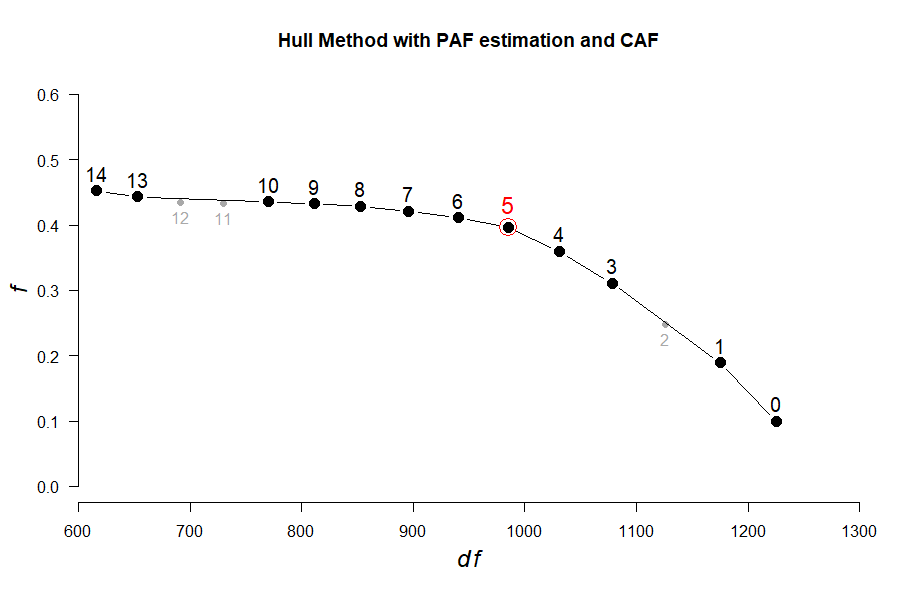
\includegraphics[width=1\linewidth]{04_figures/hull-n-factors} \caption{Results of Kaiser-Guttman criterion for determining the number of factors}\label{fig:hull-figure}
\end{figure}

\begin{figure}
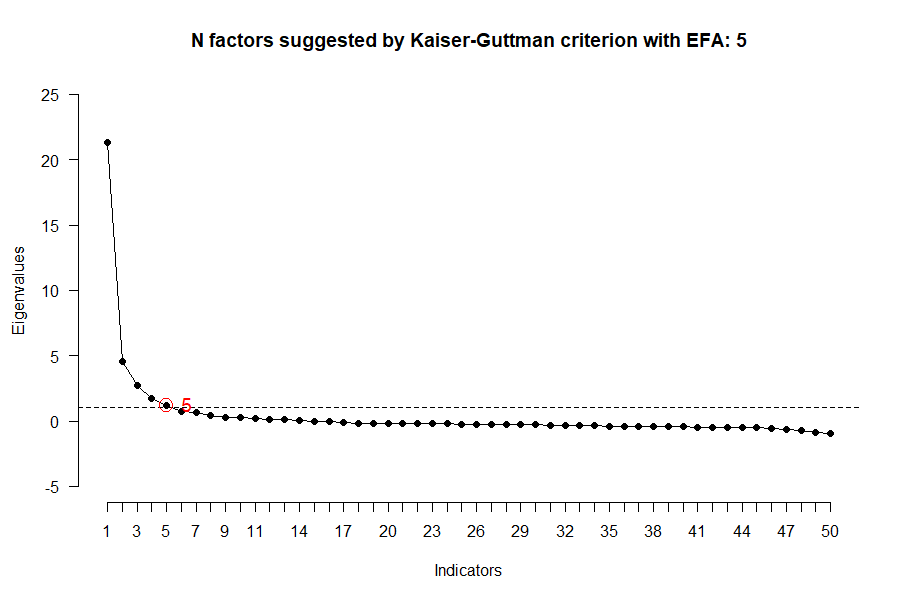
\includegraphics[width=1\linewidth]{04_figures/KGC-n-factors} \caption{Results of Hull method for determining the number of factors}\label{fig:kgc-figure}
\end{figure}

We assigned names to each factor based on a visual
inspection of the results. The \emph{drivable} factor had the highest loadings
for variables representing access by car to most destination types. The
\emph{walkable} factor has high loadings for variables representing access
by walking and transit. The \emph{diverse} index is characterized by diversity of
people (high percentages of black residents and low percentages of white
residents), diversity of land use (a greater number of distinct land
uses in the immediate vicinity and a shorter average distance to disamenities),
and lower assessed property values. The \emph{dense} factor is characterized by lower
values for the radius of the smallest buffer containing two thousand residents
(i.e.~higher population densities) and higher access to retail and grocery
locations by non-motorized modes. The \emph{amenities} factor is characterized
by non-motorized and transit access to retail and grocery locations. Figure
\ref{fig:loading-fig} illustrates the loadings of each individual variable
onto each of the five factors.

\begin{figure}
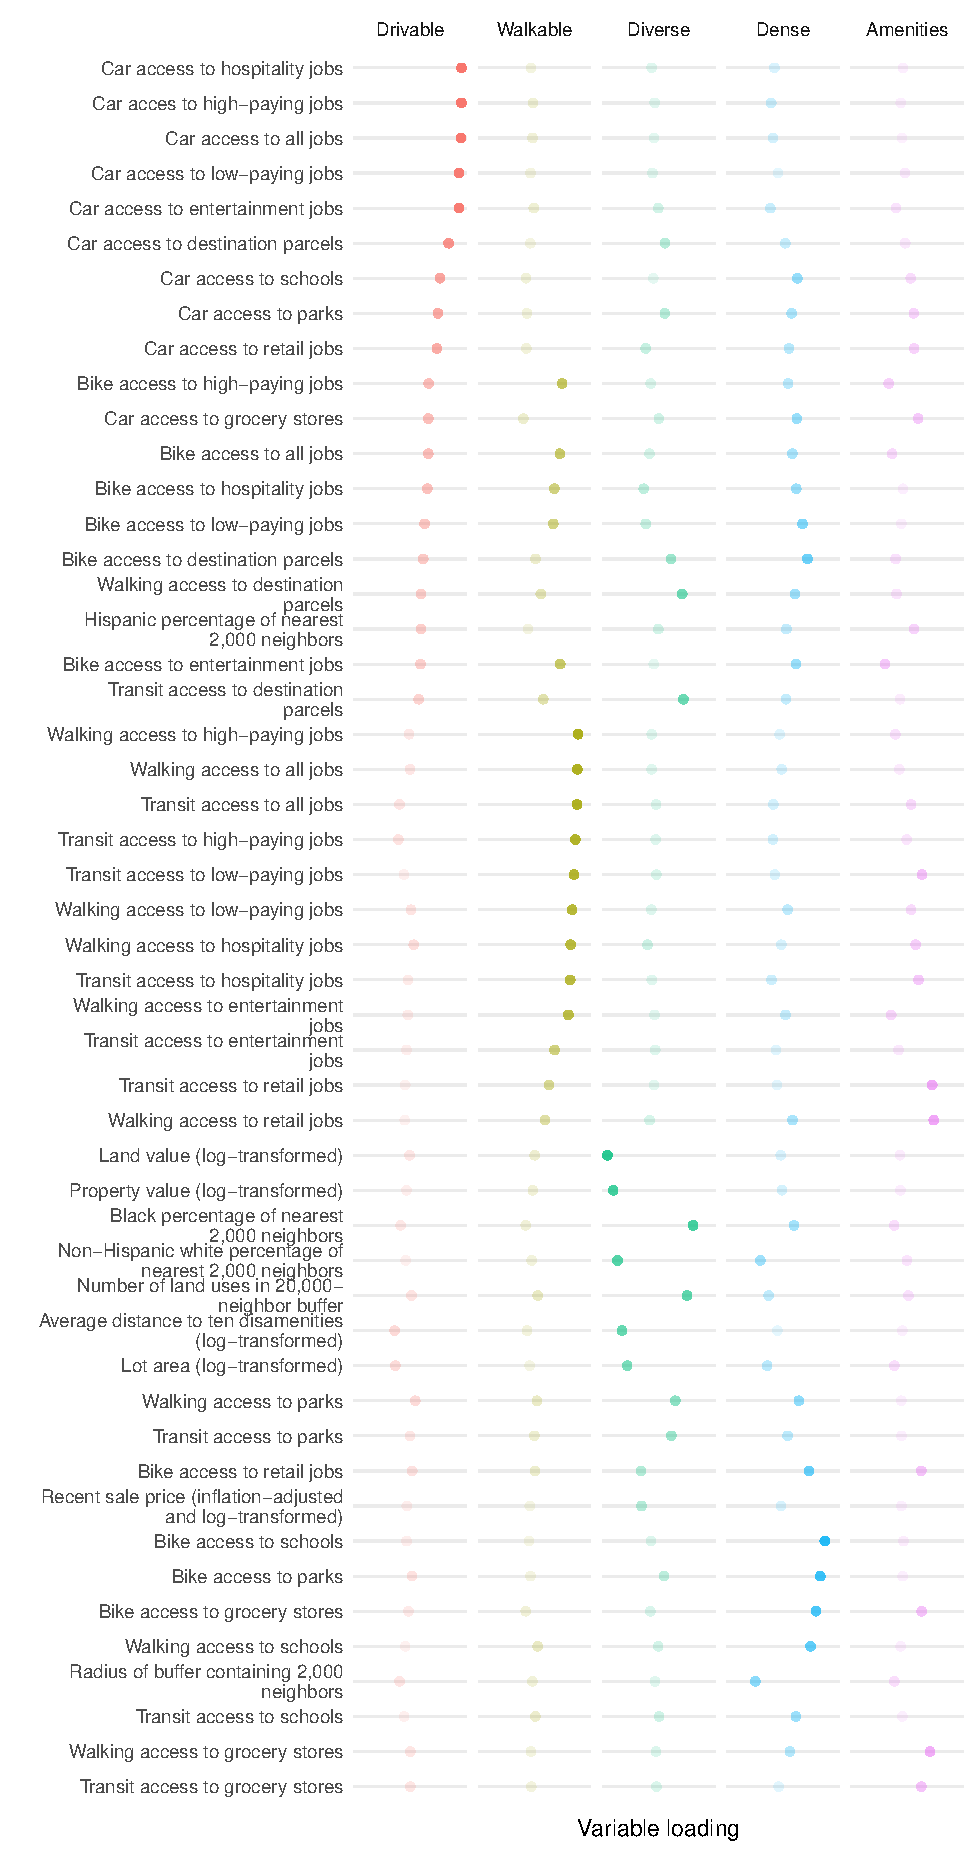
\includegraphics[width=1\linewidth]{_main_files/figure-latex/loading-fig-1} \caption{Factor loadings}\label{fig:loading-fig}
\end{figure}

\hypertarget{indices-from-factors}{%
\section{Indices from factors}\label{indices-from-factors}}

Figures \ref{fig:drive-map} through \ref{fig:amenities-map} show the spatial
variation in the drivability, walkability, density, diversity, and
amenity-richness indices, respectively.

\begin{figure}
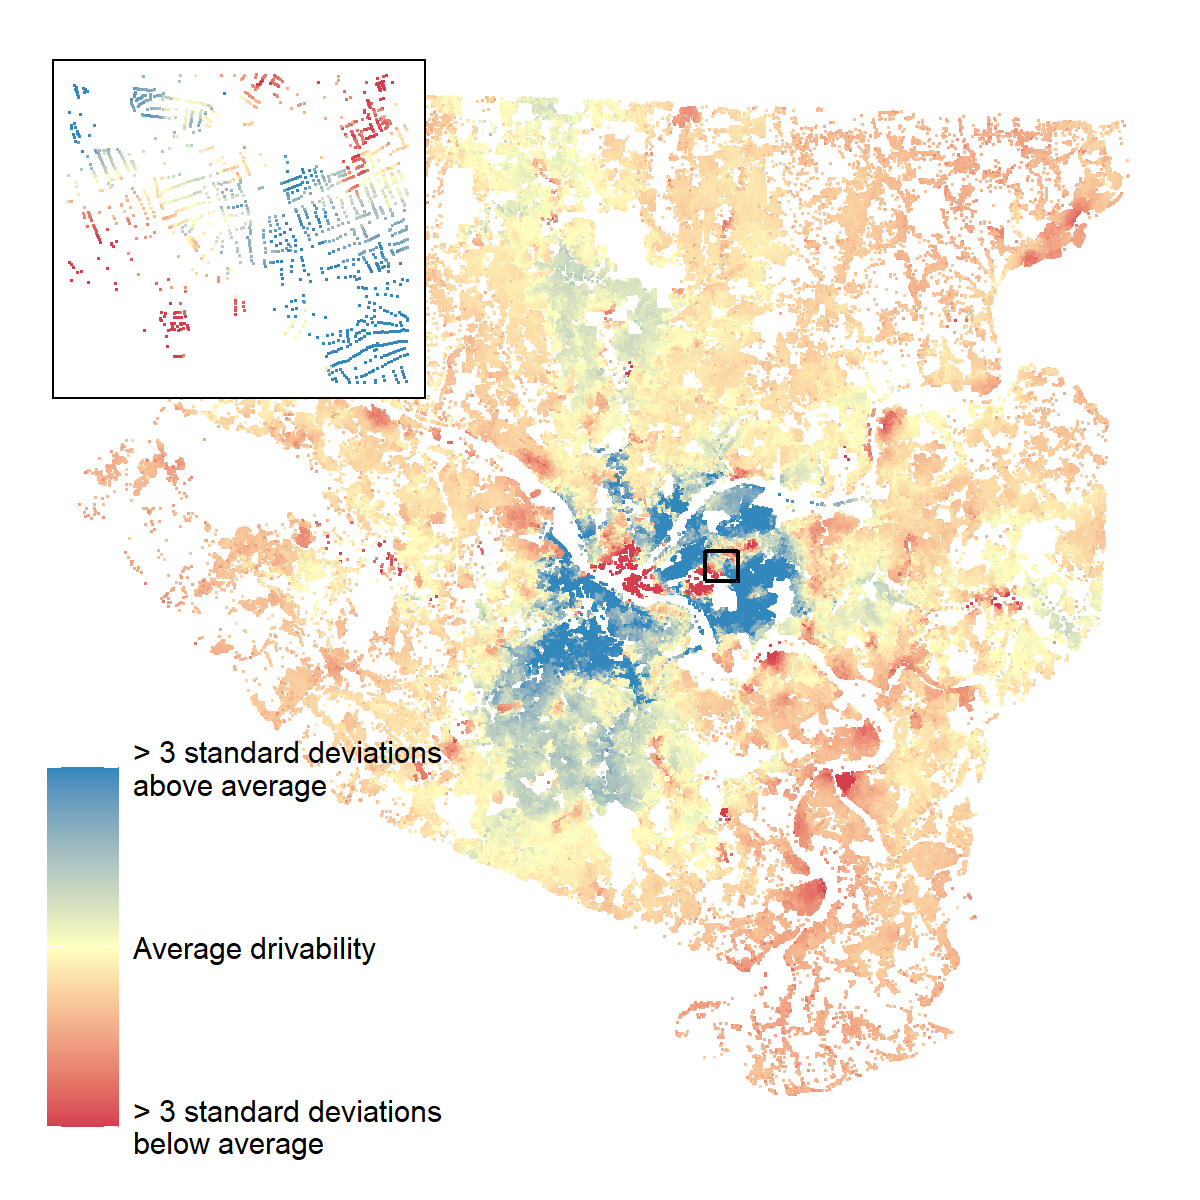
\includegraphics[width=1\linewidth]{04_figures/drivable} \caption{Spatial variation in drivability index}\label{fig:drive-map}
\end{figure}

As illistrated in Figure
\ref{fig:drive-map}, there is an area in the center of the
region (downtown Pittsburgh) with particularly low
drivablity (likely due to traffic congestion), surrounded
by a ring around the center with particularly high
drivability.

\begin{figure}
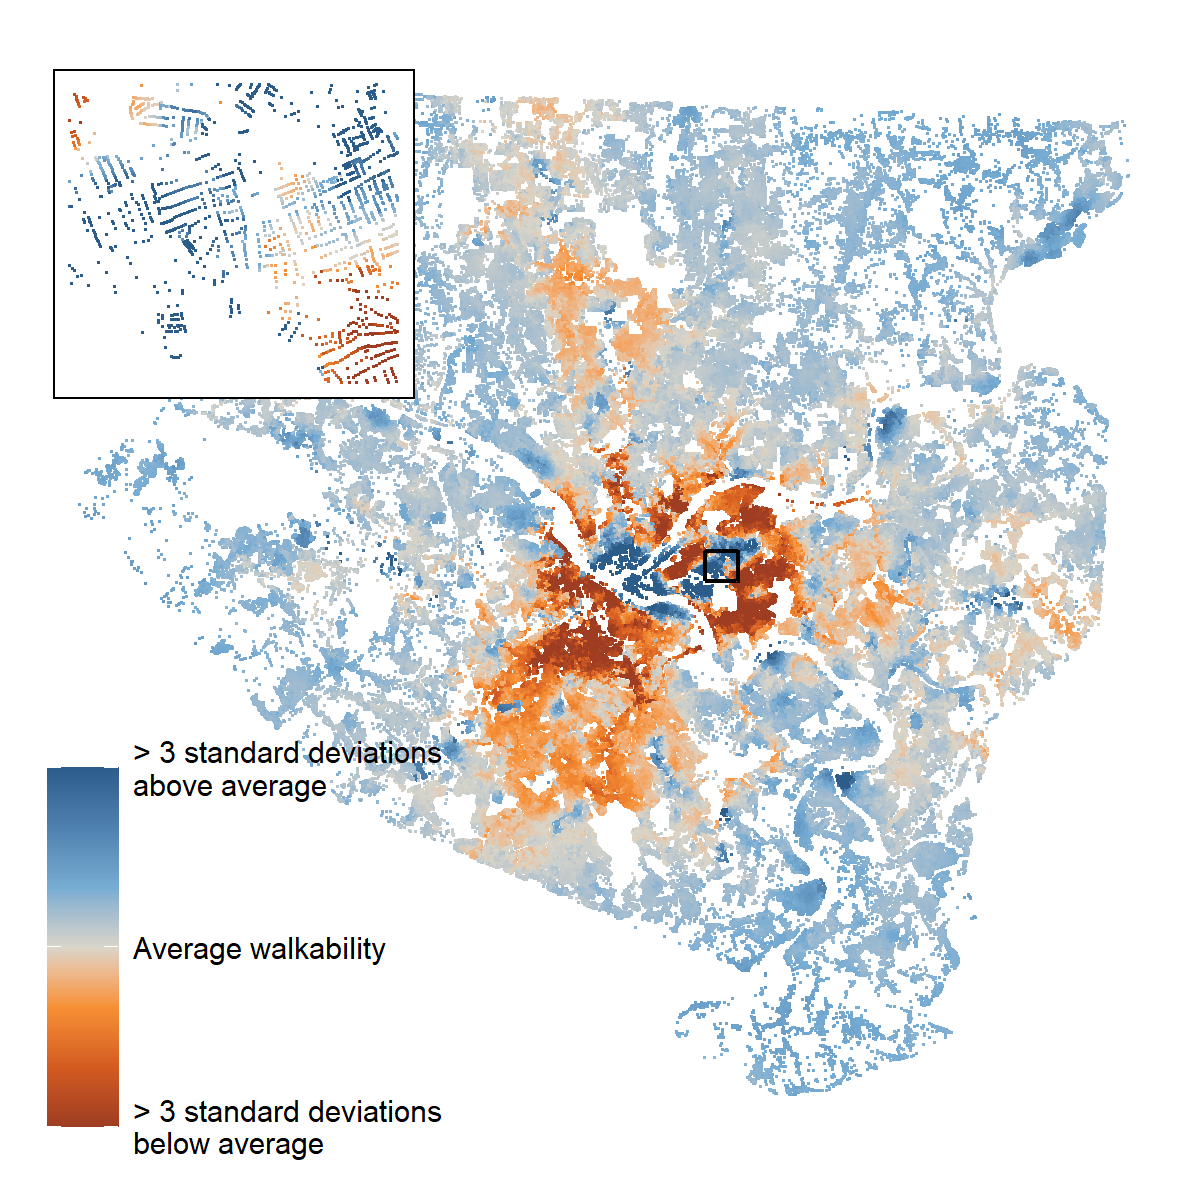
\includegraphics[width=1\linewidth]{04_figures/walkable} \caption{Spatial variation in walkability index}\label{fig:walk-map}
\end{figure}

Figure
\ref{fig:walk-map} shows the opposite pattern for walkabilty,
with particularly high walkability in the center of the
region and a ring of surrounding the center with particularly low walkability.

Figure \ref{fig:dense-map} shows pockets of low density in the
center of the region, possibly because the density index is
driven by residental density and these are commercial centers
with relatively few residents. With the exception of those
pockets, the density is generally highest in the center of the
county and lowest closer to the boundaries.

\begin{figure}
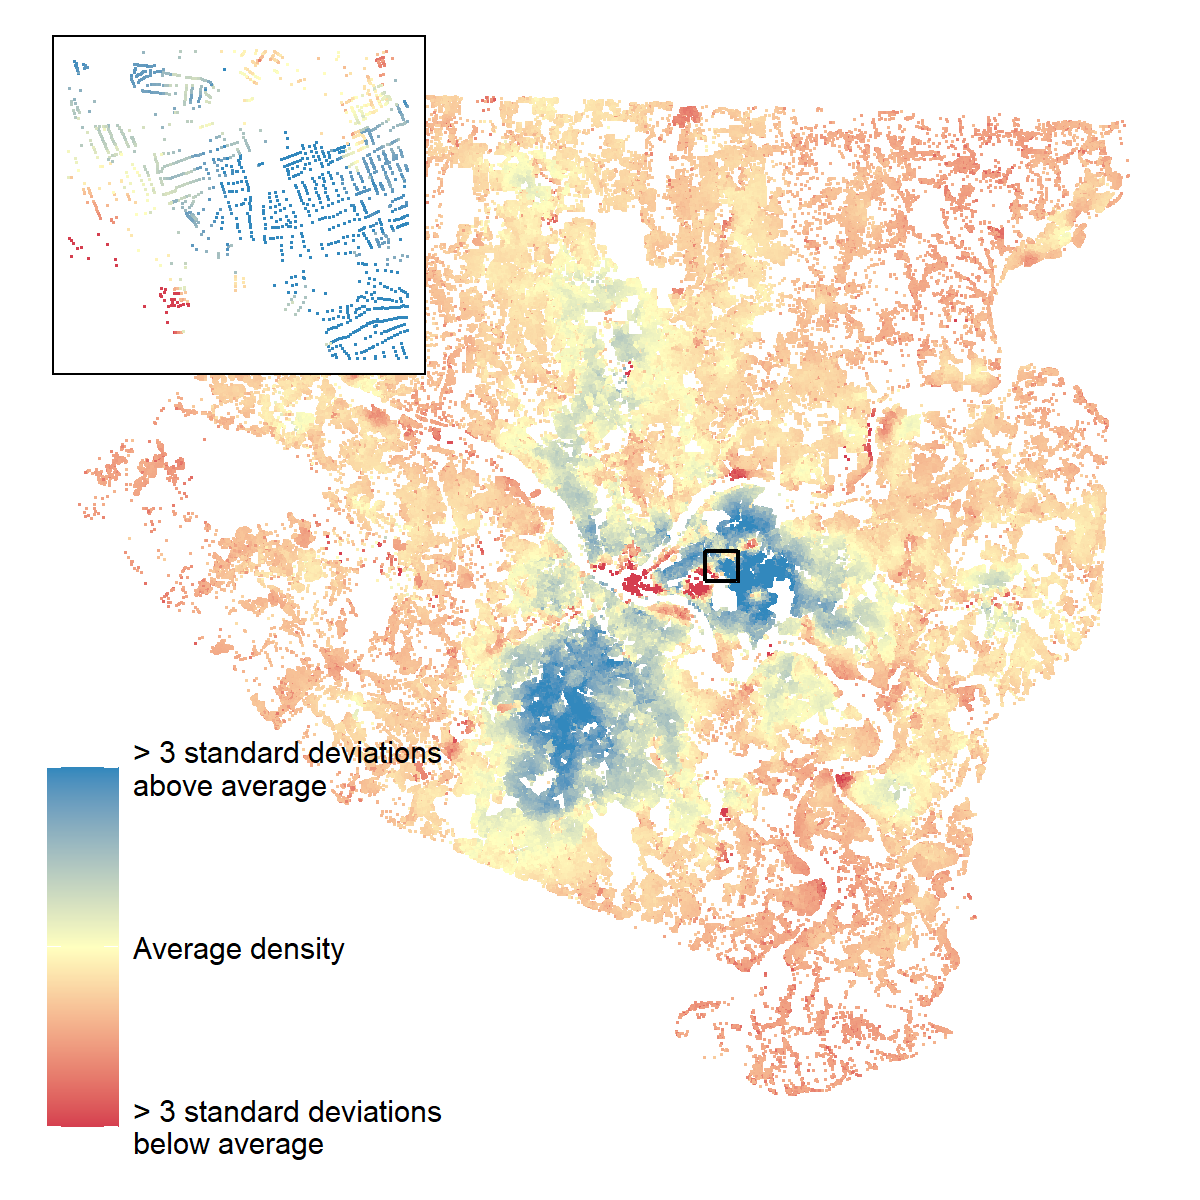
\includegraphics[width=1\linewidth]{04_figures/dense} \caption{Spatial variation in density index}\label{fig:dense-map}
\end{figure}

Figure \ref{fig:diverse-map} suggests that the greatest diversity
(with an index representing both sociodemographic and land-use
diversity) is found in areas adjacent to the center of the region.

\begin{figure}
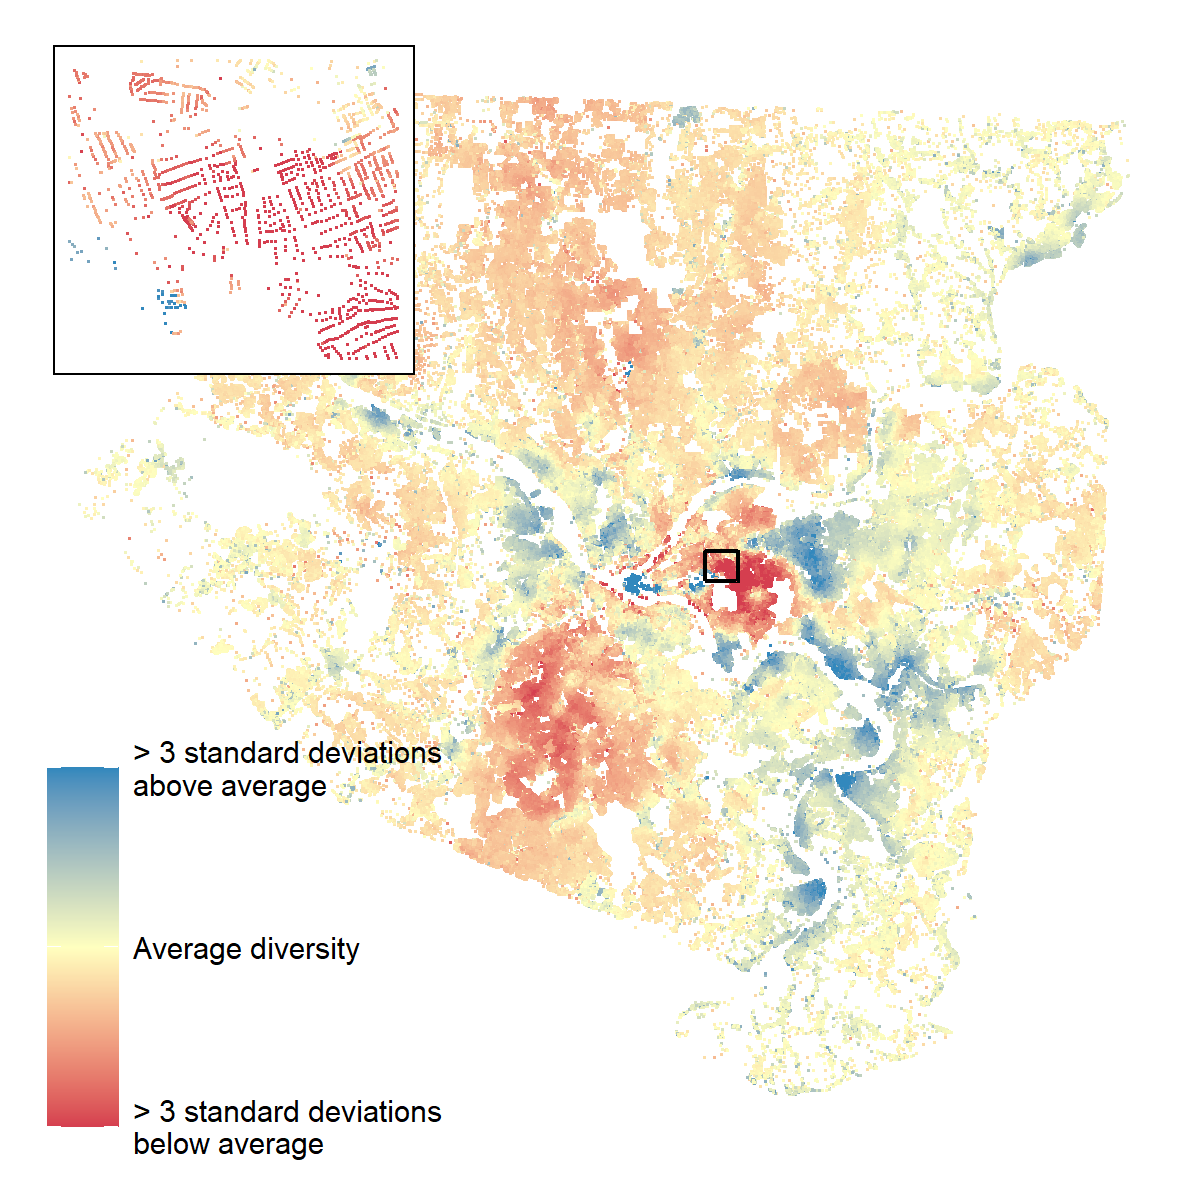
\includegraphics[width=1\linewidth]{04_figures/diverse} \caption{Spatial variation in diversity index}\label{fig:diverse-map}
\end{figure}

\begin{figure}
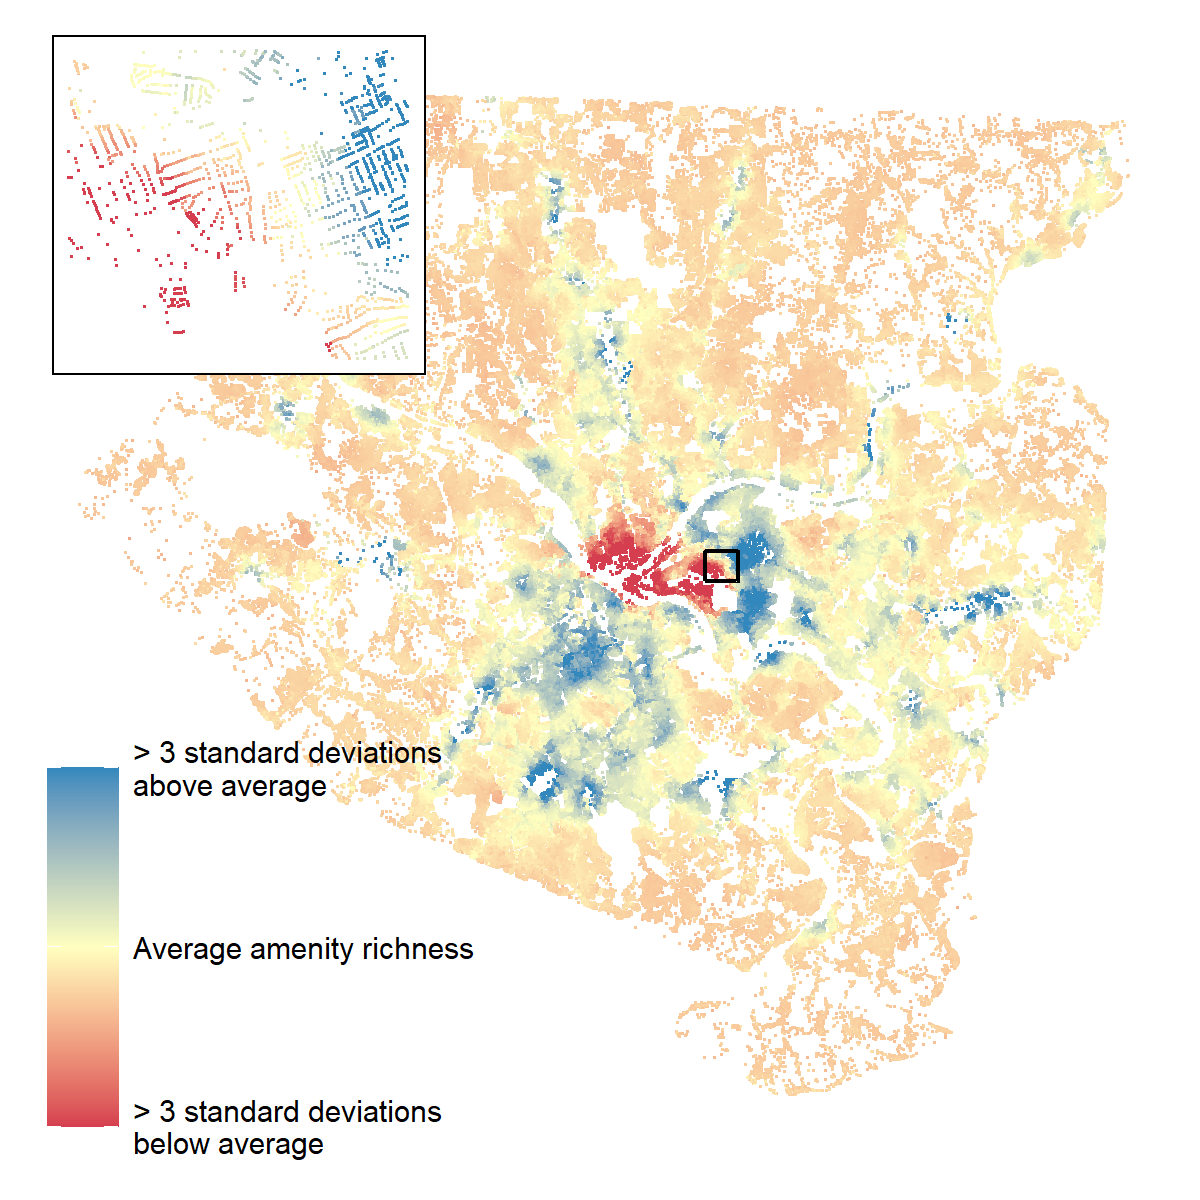
\includegraphics[width=1\linewidth]{04_figures/amenities} \caption{Spatial variation in amenity-richness index}\label{fig:amenities-map}
\end{figure}

Finally, Figure \ref{fig:amenities-map} suggests an amenity-poor
area at the center of the region surrounded by and amenity-rich ring,
with remainder of the county having an amenity richness closer to the
county average.

Figure \ref{fig:factor-cor} illustrates the distribution of each factor and the
relationships among them. In general, there appears to be a
trade-off between drivability and walkability and between drivability and diversity.
There also appears to be a negative association
between density and diversity. This may be because land-use diversity was measured
as the number of unique land uses
within the smallest buffer containing at least 2,000 residents. In very dense places,
this buffer might be too small to include a large number of unique land uses.

\begin{figure}
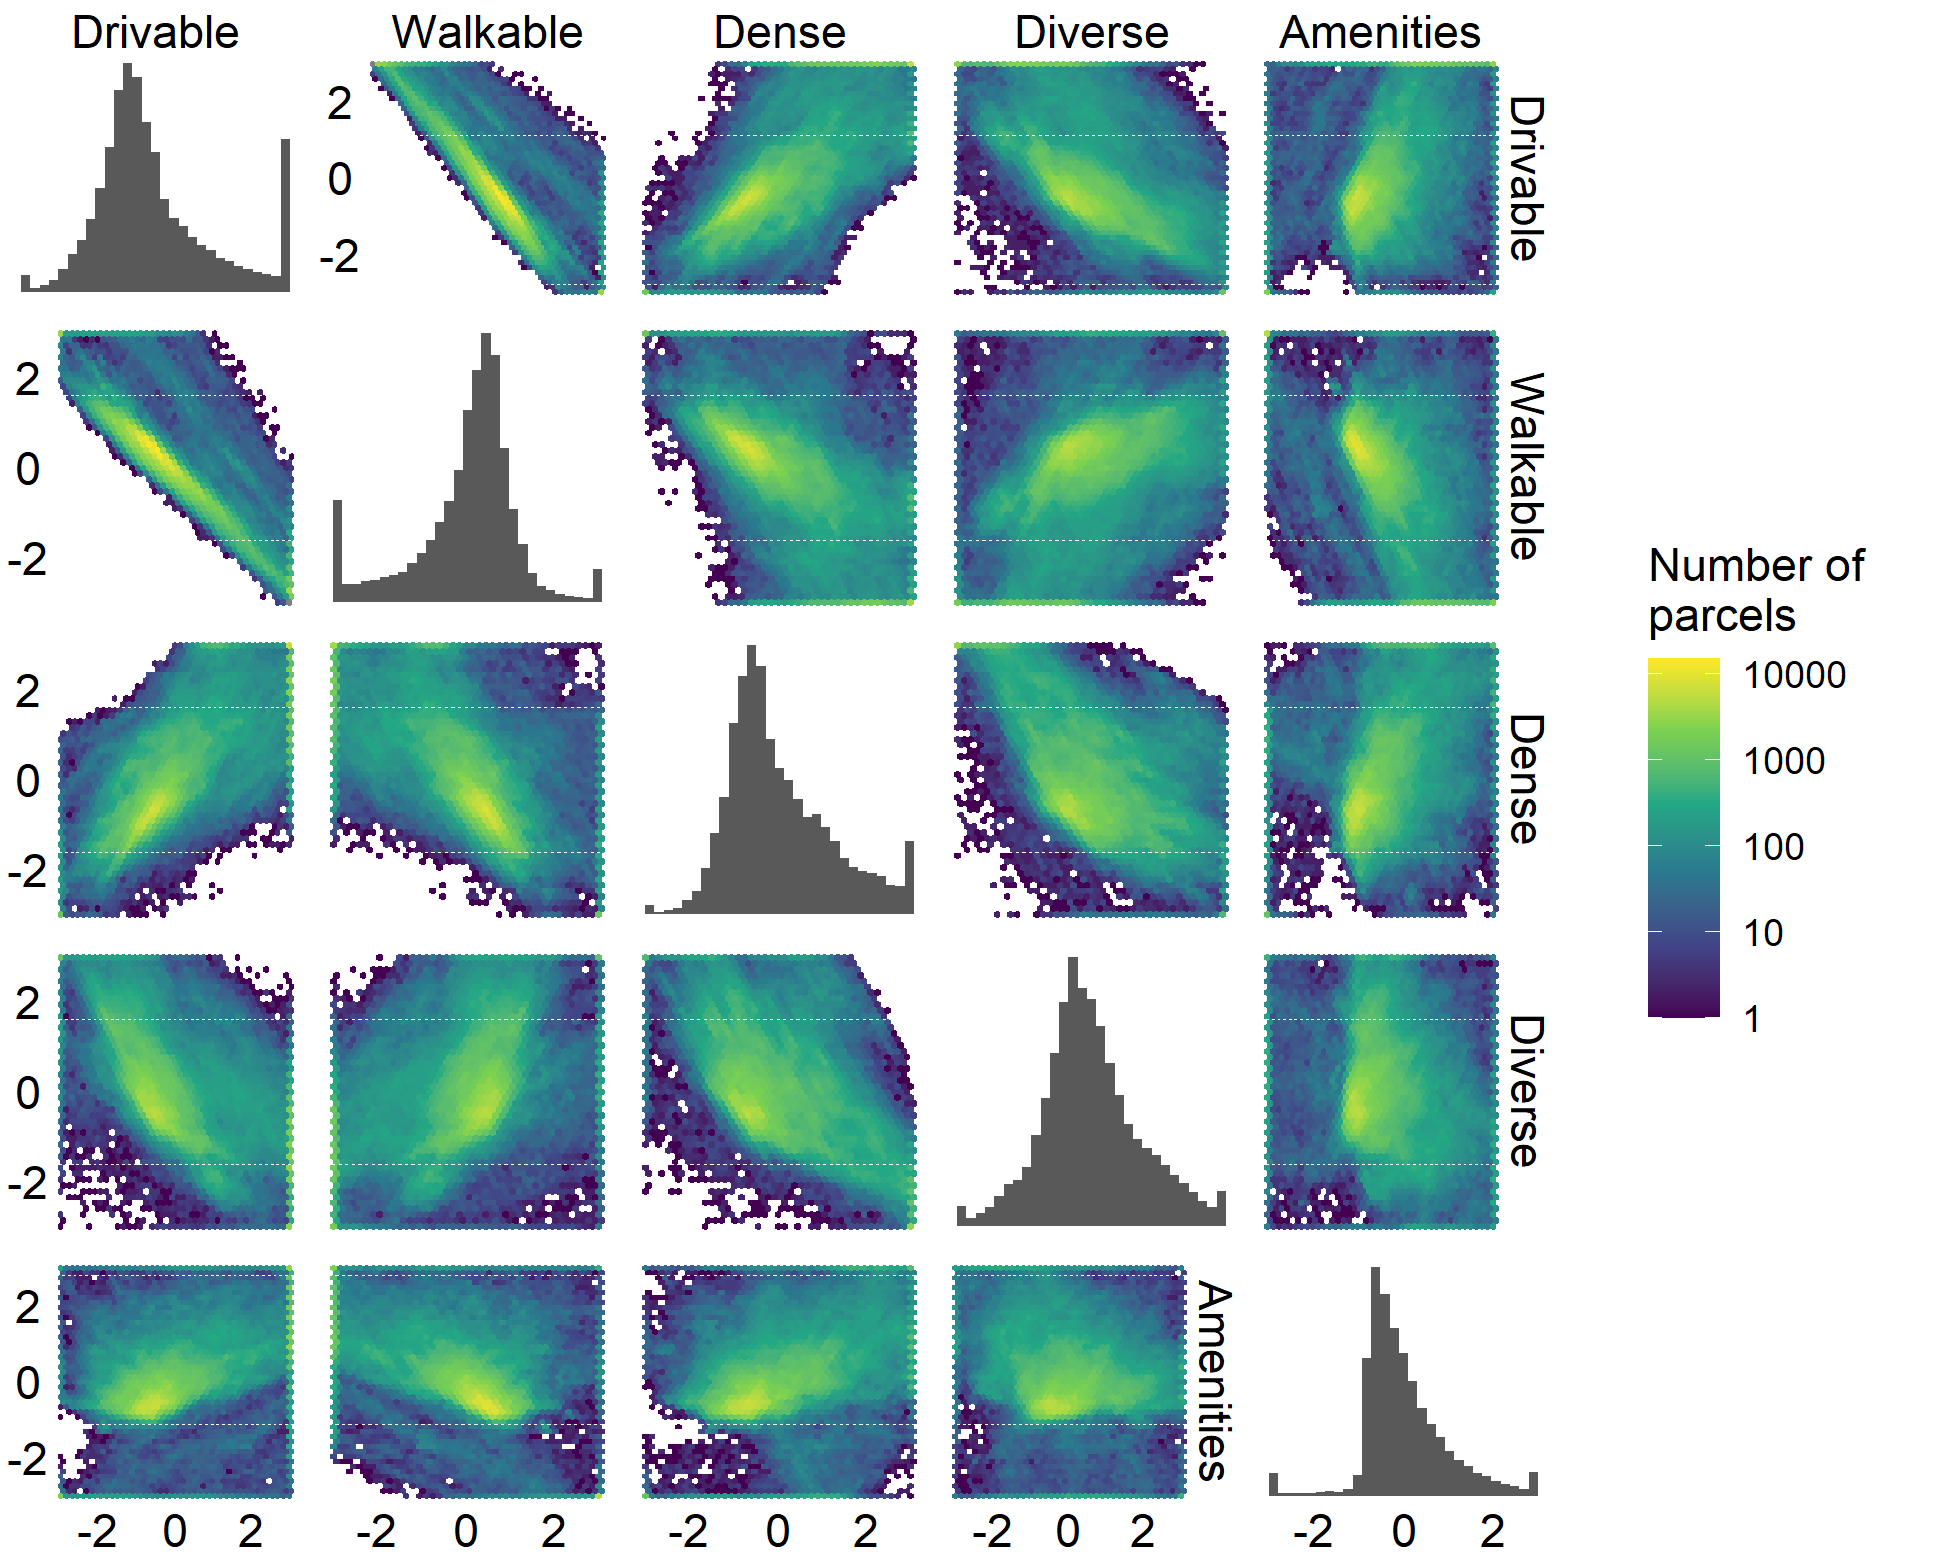
\includegraphics[width=1\linewidth]{04_figures/factor-cor} \caption{Spatial variation in amenity-richness index}\label{fig:factor-cor}
\end{figure}

\hypertarget{factor-validation-through-regression}{%
\section{Factor validation through regression}\label{factor-validation-through-regression}}

Table \ref{tab:regress} shows the results of three alternative regression models. The first of these is a
null model, which assumes that likelihood of the modeled outcome (in this case, a building permit for construction
or demolition) is constant across all sites. The second model
(labeled as the ``full model'') predicts that likelihood based
on the variation in the three indices generated by the
factor analysis. As shown, four of the five factors are
statistically significant predictors of the likelihood of
a building permit at a 99.9 percent confidence level, and this model fits the data better than the null model
based on three measures of model fit: The Akaike Information
Criterion (AIC), the Bayesian Information Criterion (BIC), and the pseudo R\^{}2. Based on the results of the full model, the amenity-richness index is not a significant predictor
of the likelihood of a building permit, so a reduced model
was estimated without that variable. In this reduced model,
the remaining model coefficients were unchanged and the
model fit was essentially unchanged.

 
  \providecommand{\huxb}[2]{\arrayrulecolor[RGB]{#1}\global\arrayrulewidth=#2pt}
  \providecommand{\huxvb}[2]{\color[RGB]{#1}\vrule width #2pt}
  \providecommand{\huxtpad}[1]{\rule{0pt}{#1}}
  \providecommand{\huxbpad}[1]{\rule[-#1]{0pt}{#1}}

\begin{table}[ht]
\begin{centerbox}
\begin{threeparttable}
\captionsetup{justification=centering,singlelinecheck=off}
\caption{\label{tab:regress} Results of logistic regression predicting likelihood of a demolition or construction permit over a one-year period.}
 \setlength{\tabcolsep}{0pt}
\begin{tabular}{l l l l}


\hhline{>{\huxb{0, 0, 0}{0.8}}->{\huxb{0, 0, 0}{0.8}}->{\huxb{0, 0, 0}{0.8}}->{\huxb{0, 0, 0}{0.8}}-}
\arrayrulecolor{black}

\multicolumn{1}{!{\huxvb{0, 0, 0}{0}}c!{\huxvb{0, 0, 0}{0}}}{\huxtpad{6pt + 1em}\centering \hspace{6pt}  \hspace{6pt}\huxbpad{6pt}} &
\multicolumn{1}{c!{\huxvb{0, 0, 0}{0}}}{\huxtpad{6pt + 1em}\centering \hspace{6pt} Null model \hspace{6pt}\huxbpad{6pt}} &
\multicolumn{1}{c!{\huxvb{0, 0, 0}{0}}}{\huxtpad{6pt + 1em}\centering \hspace{6pt} Full model \hspace{6pt}\huxbpad{6pt}} &
\multicolumn{1}{c!{\huxvb{0, 0, 0}{0}}}{\huxtpad{6pt + 1em}\centering \hspace{6pt} Reduced model \hspace{6pt}\huxbpad{6pt}} \tabularnewline[-0.5pt]


\hhline{>{\huxb{255, 255, 255}{0.4}}->{\huxb{0, 0, 0}{0.4}}->{\huxb{0, 0, 0}{0.4}}->{\huxb{0, 0, 0}{0.4}}-}
\arrayrulecolor{black}

\multicolumn{1}{!{\huxvb{0, 0, 0}{0}}l!{\huxvb{0, 0, 0}{0}}}{\huxtpad{6pt + 1em}\raggedright \hspace{6pt} (Intercept) \hspace{6pt}\huxbpad{6pt}} &
\multicolumn{1}{r!{\huxvb{0, 0, 0}{0}}}{\huxtpad{6pt + 1em}\raggedleft \hspace{6pt} -8.04 *** \hspace{6pt}\huxbpad{6pt}} &
\multicolumn{1}{r!{\huxvb{0, 0, 0}{0}}}{\huxtpad{6pt + 1em}\raggedleft \hspace{6pt} -9.57 *** \hspace{6pt}\huxbpad{6pt}} &
\multicolumn{1}{r!{\huxvb{0, 0, 0}{0}}}{\huxtpad{6pt + 1em}\raggedleft \hspace{6pt} -9.57 *** \hspace{6pt}\huxbpad{6pt}} \tabularnewline[-0.5pt]


\hhline{}
\arrayrulecolor{black}

\multicolumn{1}{!{\huxvb{0, 0, 0}{0}}l!{\huxvb{0, 0, 0}{0}}}{\huxtpad{6pt + 1em}\raggedright \hspace{6pt}  \hspace{6pt}\huxbpad{6pt}} &
\multicolumn{1}{r!{\huxvb{0, 0, 0}{0}}}{\huxtpad{6pt + 1em}\raggedleft \hspace{6pt} (SE = 0.11)\hphantom{0}\hphantom{0}\hphantom{0} \hspace{6pt}\huxbpad{6pt}} &
\multicolumn{1}{r!{\huxvb{0, 0, 0}{0}}}{\huxtpad{6pt + 1em}\raggedleft \hspace{6pt} (SE = 0.25)\hphantom{0}\hphantom{0}\hphantom{0} \hspace{6pt}\huxbpad{6pt}} &
\multicolumn{1}{r!{\huxvb{0, 0, 0}{0}}}{\huxtpad{6pt + 1em}\raggedleft \hspace{6pt} (SE = 0.24)\hphantom{0}\hphantom{0}\hphantom{0} \hspace{6pt}\huxbpad{6pt}} \tabularnewline[-0.5pt]


\hhline{}
\arrayrulecolor{black}

\multicolumn{1}{!{\huxvb{0, 0, 0}{0}}l!{\huxvb{0, 0, 0}{0}}}{\huxtpad{6pt + 1em}\raggedright \hspace{6pt} Drivable \hspace{6pt}\huxbpad{6pt}} &
\multicolumn{1}{r!{\huxvb{0, 0, 0}{0}}}{\huxtpad{6pt + 1em}\raggedleft \hspace{6pt} \hphantom{0}\hphantom{0}\hphantom{0}\hphantom{0}\hphantom{0}\hphantom{0}\hphantom{0} \hspace{6pt}\huxbpad{6pt}} &
\multicolumn{1}{r!{\huxvb{0, 0, 0}{0}}}{\huxtpad{6pt + 1em}\raggedleft \hspace{6pt} 1.35 *** \hspace{6pt}\huxbpad{6pt}} &
\multicolumn{1}{r!{\huxvb{0, 0, 0}{0}}}{\huxtpad{6pt + 1em}\raggedleft \hspace{6pt} 1.35 *** \hspace{6pt}\huxbpad{6pt}} \tabularnewline[-0.5pt]


\hhline{}
\arrayrulecolor{black}

\multicolumn{1}{!{\huxvb{0, 0, 0}{0}}l!{\huxvb{0, 0, 0}{0}}}{\huxtpad{6pt + 1em}\raggedright \hspace{6pt}  \hspace{6pt}\huxbpad{6pt}} &
\multicolumn{1}{r!{\huxvb{0, 0, 0}{0}}}{\huxtpad{6pt + 1em}\raggedleft \hspace{6pt} \hphantom{0}\hphantom{0}\hphantom{0}\hphantom{0}\hphantom{0}\hphantom{0}\hphantom{0} \hspace{6pt}\huxbpad{6pt}} &
\multicolumn{1}{r!{\huxvb{0, 0, 0}{0}}}{\huxtpad{6pt + 1em}\raggedleft \hspace{6pt} (SE = 0.16)\hphantom{0}\hphantom{0}\hphantom{0} \hspace{6pt}\huxbpad{6pt}} &
\multicolumn{1}{r!{\huxvb{0, 0, 0}{0}}}{\huxtpad{6pt + 1em}\raggedleft \hspace{6pt} (SE = 0.14)\hphantom{0}\hphantom{0}\hphantom{0} \hspace{6pt}\huxbpad{6pt}} \tabularnewline[-0.5pt]


\hhline{}
\arrayrulecolor{black}

\multicolumn{1}{!{\huxvb{0, 0, 0}{0}}l!{\huxvb{0, 0, 0}{0}}}{\huxtpad{6pt + 1em}\raggedright \hspace{6pt} Walkable \hspace{6pt}\huxbpad{6pt}} &
\multicolumn{1}{r!{\huxvb{0, 0, 0}{0}}}{\huxtpad{6pt + 1em}\raggedleft \hspace{6pt} \hphantom{0}\hphantom{0}\hphantom{0}\hphantom{0}\hphantom{0}\hphantom{0}\hphantom{0} \hspace{6pt}\huxbpad{6pt}} &
\multicolumn{1}{r!{\huxvb{0, 0, 0}{0}}}{\huxtpad{6pt + 1em}\raggedleft \hspace{6pt} 1.38 *** \hspace{6pt}\huxbpad{6pt}} &
\multicolumn{1}{r!{\huxvb{0, 0, 0}{0}}}{\huxtpad{6pt + 1em}\raggedleft \hspace{6pt} 1.38 *** \hspace{6pt}\huxbpad{6pt}} \tabularnewline[-0.5pt]


\hhline{}
\arrayrulecolor{black}

\multicolumn{1}{!{\huxvb{0, 0, 0}{0}}l!{\huxvb{0, 0, 0}{0}}}{\huxtpad{6pt + 1em}\raggedright \hspace{6pt}  \hspace{6pt}\huxbpad{6pt}} &
\multicolumn{1}{r!{\huxvb{0, 0, 0}{0}}}{\huxtpad{6pt + 1em}\raggedleft \hspace{6pt} \hphantom{0}\hphantom{0}\hphantom{0}\hphantom{0}\hphantom{0}\hphantom{0}\hphantom{0} \hspace{6pt}\huxbpad{6pt}} &
\multicolumn{1}{r!{\huxvb{0, 0, 0}{0}}}{\huxtpad{6pt + 1em}\raggedleft \hspace{6pt} (SE = 0.15)\hphantom{0}\hphantom{0}\hphantom{0} \hspace{6pt}\huxbpad{6pt}} &
\multicolumn{1}{r!{\huxvb{0, 0, 0}{0}}}{\huxtpad{6pt + 1em}\raggedleft \hspace{6pt} (SE = 0.11)\hphantom{0}\hphantom{0}\hphantom{0} \hspace{6pt}\huxbpad{6pt}} \tabularnewline[-0.5pt]


\hhline{}
\arrayrulecolor{black}

\multicolumn{1}{!{\huxvb{0, 0, 0}{0}}l!{\huxvb{0, 0, 0}{0}}}{\huxtpad{6pt + 1em}\raggedright \hspace{6pt} Dense \hspace{6pt}\huxbpad{6pt}} &
\multicolumn{1}{r!{\huxvb{0, 0, 0}{0}}}{\huxtpad{6pt + 1em}\raggedleft \hspace{6pt} \hphantom{0}\hphantom{0}\hphantom{0}\hphantom{0}\hphantom{0}\hphantom{0}\hphantom{0} \hspace{6pt}\huxbpad{6pt}} &
\multicolumn{1}{r!{\huxvb{0, 0, 0}{0}}}{\huxtpad{6pt + 1em}\raggedleft \hspace{6pt} 0.90 *** \hspace{6pt}\huxbpad{6pt}} &
\multicolumn{1}{r!{\huxvb{0, 0, 0}{0}}}{\huxtpad{6pt + 1em}\raggedleft \hspace{6pt} 0.90 *** \hspace{6pt}\huxbpad{6pt}} \tabularnewline[-0.5pt]


\hhline{}
\arrayrulecolor{black}

\multicolumn{1}{!{\huxvb{0, 0, 0}{0}}l!{\huxvb{0, 0, 0}{0}}}{\huxtpad{6pt + 1em}\raggedright \hspace{6pt}  \hspace{6pt}\huxbpad{6pt}} &
\multicolumn{1}{r!{\huxvb{0, 0, 0}{0}}}{\huxtpad{6pt + 1em}\raggedleft \hspace{6pt} \hphantom{0}\hphantom{0}\hphantom{0}\hphantom{0}\hphantom{0}\hphantom{0}\hphantom{0} \hspace{6pt}\huxbpad{6pt}} &
\multicolumn{1}{r!{\huxvb{0, 0, 0}{0}}}{\huxtpad{6pt + 1em}\raggedleft \hspace{6pt} (SE = 0.12)\hphantom{0}\hphantom{0}\hphantom{0} \hspace{6pt}\huxbpad{6pt}} &
\multicolumn{1}{r!{\huxvb{0, 0, 0}{0}}}{\huxtpad{6pt + 1em}\raggedleft \hspace{6pt} (SE = 0.12)\hphantom{0}\hphantom{0}\hphantom{0} \hspace{6pt}\huxbpad{6pt}} \tabularnewline[-0.5pt]


\hhline{}
\arrayrulecolor{black}

\multicolumn{1}{!{\huxvb{0, 0, 0}{0}}l!{\huxvb{0, 0, 0}{0}}}{\huxtpad{6pt + 1em}\raggedright \hspace{6pt} Diverse \hspace{6pt}\huxbpad{6pt}} &
\multicolumn{1}{r!{\huxvb{0, 0, 0}{0}}}{\huxtpad{6pt + 1em}\raggedleft \hspace{6pt} \hphantom{0}\hphantom{0}\hphantom{0}\hphantom{0}\hphantom{0}\hphantom{0}\hphantom{0} \hspace{6pt}\huxbpad{6pt}} &
\multicolumn{1}{r!{\huxvb{0, 0, 0}{0}}}{\huxtpad{6pt + 1em}\raggedleft \hspace{6pt} 0.98 *** \hspace{6pt}\huxbpad{6pt}} &
\multicolumn{1}{r!{\huxvb{0, 0, 0}{0}}}{\huxtpad{6pt + 1em}\raggedleft \hspace{6pt} 0.98 *** \hspace{6pt}\huxbpad{6pt}} \tabularnewline[-0.5pt]


\hhline{}
\arrayrulecolor{black}

\multicolumn{1}{!{\huxvb{0, 0, 0}{0}}l!{\huxvb{0, 0, 0}{0}}}{\huxtpad{6pt + 1em}\raggedright \hspace{6pt}  \hspace{6pt}\huxbpad{6pt}} &
\multicolumn{1}{r!{\huxvb{0, 0, 0}{0}}}{\huxtpad{6pt + 1em}\raggedleft \hspace{6pt} \hphantom{0}\hphantom{0}\hphantom{0}\hphantom{0}\hphantom{0}\hphantom{0}\hphantom{0} \hspace{6pt}\huxbpad{6pt}} &
\multicolumn{1}{r!{\huxvb{0, 0, 0}{0}}}{\huxtpad{6pt + 1em}\raggedleft \hspace{6pt} (SE = 0.12)\hphantom{0}\hphantom{0}\hphantom{0} \hspace{6pt}\huxbpad{6pt}} &
\multicolumn{1}{r!{\huxvb{0, 0, 0}{0}}}{\huxtpad{6pt + 1em}\raggedleft \hspace{6pt} (SE = 0.11)\hphantom{0}\hphantom{0}\hphantom{0} \hspace{6pt}\huxbpad{6pt}} \tabularnewline[-0.5pt]


\hhline{}
\arrayrulecolor{black}

\multicolumn{1}{!{\huxvb{0, 0, 0}{0}}l!{\huxvb{0, 0, 0}{0}}}{\huxtpad{6pt + 1em}\raggedright \hspace{6pt} Amenities \hspace{6pt}\huxbpad{6pt}} &
\multicolumn{1}{r!{\huxvb{0, 0, 0}{0}}}{\huxtpad{6pt + 1em}\raggedleft \hspace{6pt} \hphantom{0}\hphantom{0}\hphantom{0}\hphantom{0}\hphantom{0}\hphantom{0}\hphantom{0} \hspace{6pt}\huxbpad{6pt}} &
\multicolumn{1}{r!{\huxvb{0, 0, 0}{0}}}{\huxtpad{6pt + 1em}\raggedleft \hspace{6pt} 0.00\hphantom{0}\hphantom{0}\hphantom{0}\hphantom{0} \hspace{6pt}\huxbpad{6pt}} &
\multicolumn{1}{r!{\huxvb{0, 0, 0}{0}}}{\huxtpad{6pt + 1em}\raggedleft \hspace{6pt} \hphantom{0}\hphantom{0}\hphantom{0}\hphantom{0}\hphantom{0}\hphantom{0}\hphantom{0} \hspace{6pt}\huxbpad{6pt}} \tabularnewline[-0.5pt]


\hhline{}
\arrayrulecolor{black}

\multicolumn{1}{!{\huxvb{0, 0, 0}{0}}l!{\huxvb{0, 0, 0}{0}}}{\huxtpad{6pt + 1em}\raggedright \hspace{6pt}  \hspace{6pt}\huxbpad{6pt}} &
\multicolumn{1}{r!{\huxvb{0, 0, 0}{0}}}{\huxtpad{6pt + 1em}\raggedleft \hspace{6pt} \hphantom{0}\hphantom{0}\hphantom{0}\hphantom{0}\hphantom{0}\hphantom{0}\hphantom{0} \hspace{6pt}\huxbpad{6pt}} &
\multicolumn{1}{r!{\huxvb{0, 0, 0}{0}}}{\huxtpad{6pt + 1em}\raggedleft \hspace{6pt} (SE = 0.07)\hphantom{0}\hphantom{0}\hphantom{0} \hspace{6pt}\huxbpad{6pt}} &
\multicolumn{1}{r!{\huxvb{0, 0, 0}{0}}}{\huxtpad{6pt + 1em}\raggedleft \hspace{6pt} \hphantom{0}\hphantom{0}\hphantom{0}\hphantom{0}\hphantom{0}\hphantom{0}\hphantom{0} \hspace{6pt}\huxbpad{6pt}} \tabularnewline[-0.5pt]


\hhline{>{\huxb{255, 255, 255}{0.4}}->{\huxb{0, 0, 0}{0.4}}->{\huxb{0, 0, 0}{0.4}}->{\huxb{0, 0, 0}{0.4}}-}
\arrayrulecolor{black}

\multicolumn{1}{!{\huxvb{0, 0, 0}{0}}l!{\huxvb{0, 0, 0}{0}}}{\huxtpad{6pt + 1em}\raggedright \hspace{6pt} N \hspace{6pt}\huxbpad{6pt}} &
\multicolumn{1}{r!{\huxvb{0, 0, 0}{0}}}{\huxtpad{6pt + 1em}\raggedleft \hspace{6pt} 269151\hphantom{0}\hphantom{0}\hphantom{0}\hphantom{0}\hphantom{0}\hphantom{0}\hphantom{0} \hspace{6pt}\huxbpad{6pt}} &
\multicolumn{1}{r!{\huxvb{0, 0, 0}{0}}}{\huxtpad{6pt + 1em}\raggedleft \hspace{6pt} 269151\hphantom{0}\hphantom{0}\hphantom{0}\hphantom{0}\hphantom{0}\hphantom{0}\hphantom{0} \hspace{6pt}\huxbpad{6pt}} &
\multicolumn{1}{r!{\huxvb{0, 0, 0}{0}}}{\huxtpad{6pt + 1em}\raggedleft \hspace{6pt} 269151\hphantom{0}\hphantom{0}\hphantom{0}\hphantom{0}\hphantom{0}\hphantom{0}\hphantom{0} \hspace{6pt}\huxbpad{6pt}} \tabularnewline[-0.5pt]


\hhline{}
\arrayrulecolor{black}

\multicolumn{1}{!{\huxvb{0, 0, 0}{0}}l!{\huxvb{0, 0, 0}{0}}}{\huxtpad{6pt + 1em}\raggedright \hspace{6pt} AIC \hspace{6pt}\huxbpad{6pt}} &
\multicolumn{1}{r!{\huxvb{0, 0, 0}{0}}}{\huxtpad{6pt + 1em}\raggedleft \hspace{6pt} 1574.43\hphantom{0}\hphantom{0}\hphantom{0}\hphantom{0} \hspace{6pt}\huxbpad{6pt}} &
\multicolumn{1}{r!{\huxvb{0, 0, 0}{0}}}{\huxtpad{6pt + 1em}\raggedleft \hspace{6pt} 1414.33\hphantom{0}\hphantom{0}\hphantom{0}\hphantom{0} \hspace{6pt}\huxbpad{6pt}} &
\multicolumn{1}{r!{\huxvb{0, 0, 0}{0}}}{\huxtpad{6pt + 1em}\raggedleft \hspace{6pt} 1412.33\hphantom{0}\hphantom{0}\hphantom{0}\hphantom{0} \hspace{6pt}\huxbpad{6pt}} \tabularnewline[-0.5pt]


\hhline{}
\arrayrulecolor{black}

\multicolumn{1}{!{\huxvb{0, 0, 0}{0}}l!{\huxvb{0, 0, 0}{0}}}{\huxtpad{6pt + 1em}\raggedright \hspace{6pt} BIC \hspace{6pt}\huxbpad{6pt}} &
\multicolumn{1}{r!{\huxvb{0, 0, 0}{0}}}{\huxtpad{6pt + 1em}\raggedleft \hspace{6pt} 1584.93\hphantom{0}\hphantom{0}\hphantom{0}\hphantom{0} \hspace{6pt}\huxbpad{6pt}} &
\multicolumn{1}{r!{\huxvb{0, 0, 0}{0}}}{\huxtpad{6pt + 1em}\raggedleft \hspace{6pt} 1477.35\hphantom{0}\hphantom{0}\hphantom{0}\hphantom{0} \hspace{6pt}\huxbpad{6pt}} &
\multicolumn{1}{r!{\huxvb{0, 0, 0}{0}}}{\huxtpad{6pt + 1em}\raggedleft \hspace{6pt} 1464.84\hphantom{0}\hphantom{0}\hphantom{0}\hphantom{0} \hspace{6pt}\huxbpad{6pt}} \tabularnewline[-0.5pt]


\hhline{}
\arrayrulecolor{black}

\multicolumn{1}{!{\huxvb{0, 0, 0}{0}}l!{\huxvb{0, 0, 0}{0}}}{\huxtpad{6pt + 1em}\raggedright \hspace{6pt} Pseudo R2 \hspace{6pt}\huxbpad{6pt}} &
\multicolumn{1}{r!{\huxvb{0, 0, 0}{0}}}{\huxtpad{6pt + 1em}\raggedleft \hspace{6pt} 0.00\hphantom{0}\hphantom{0}\hphantom{0}\hphantom{0} \hspace{6pt}\huxbpad{6pt}} &
\multicolumn{1}{r!{\huxvb{0, 0, 0}{0}}}{\huxtpad{6pt + 1em}\raggedleft \hspace{6pt} 0.11\hphantom{0}\hphantom{0}\hphantom{0}\hphantom{0} \hspace{6pt}\huxbpad{6pt}} &
\multicolumn{1}{r!{\huxvb{0, 0, 0}{0}}}{\huxtpad{6pt + 1em}\raggedleft \hspace{6pt} 0.11\hphantom{0}\hphantom{0}\hphantom{0}\hphantom{0} \hspace{6pt}\huxbpad{6pt}} \tabularnewline[-0.5pt]


\hhline{>{\huxb{0, 0, 0}{0.8}}->{\huxb{0, 0, 0}{0.8}}->{\huxb{0, 0, 0}{0.8}}->{\huxb{0, 0, 0}{0.8}}-}
\arrayrulecolor{black}

\multicolumn{4}{!{\huxvb{0, 0, 0}{0}}l!{\huxvb{0, 0, 0}{0}}}{\huxtpad{6pt + 1em}\raggedright \hspace{6pt}  *** p $<$ 0.001;  ** p $<$ 0.01;  * p $<$ 0.05. \hspace{6pt}\huxbpad{6pt}} \tabularnewline[-0.5pt]


\hhline{}
\arrayrulecolor{black}
\end{tabular}
\end{threeparttable}\par\end{centerbox}

\end{table}
 

Figure \ref{fig:effect-plot} shows how the predicted probability
of development changes as each index varies from -5 to 5
(i.e.~from five standard deviations below the average to
five standard deviations above the average).

\begin{figure}
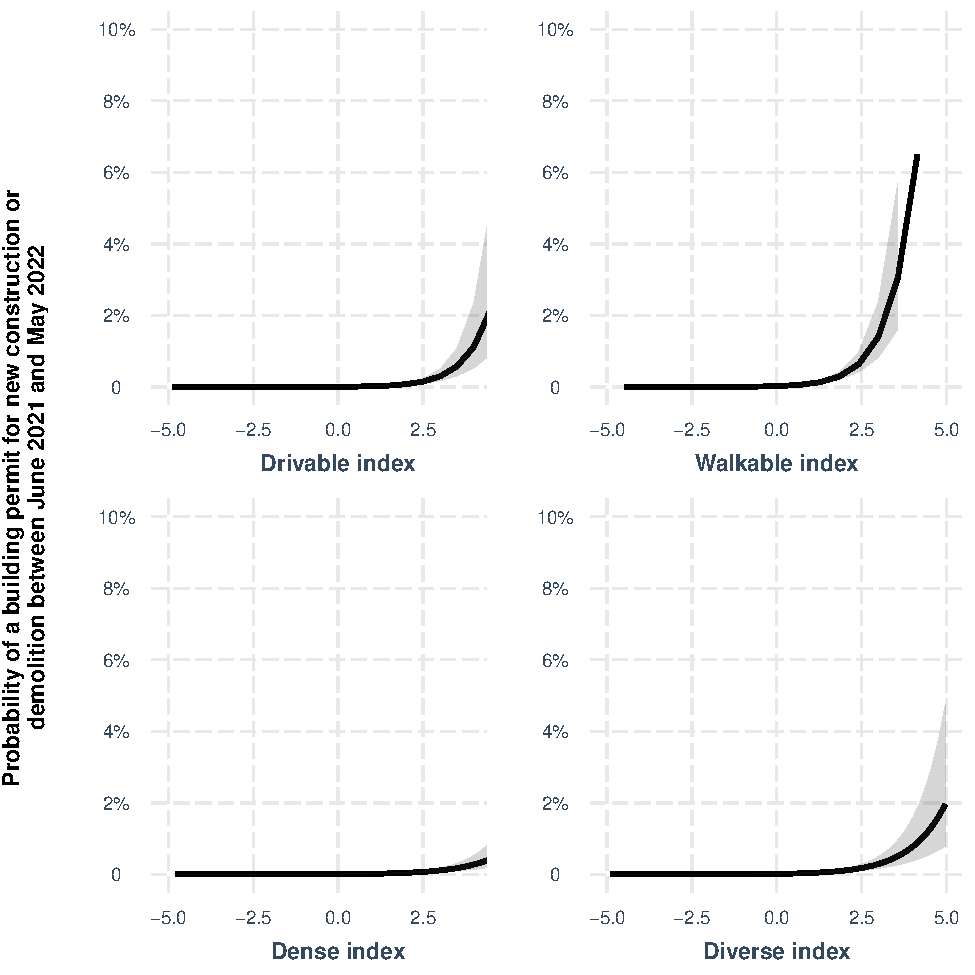
\includegraphics[width=1\linewidth]{_main_files/figure-latex/effect-plot-1} \caption{Effect of drivability, walkabilty, diversity, and density on development probability}\label{fig:effect-plot}
\end{figure}

\hypertarget{combined-index-1}{%
\section{Combined index}\label{combined-index-1}}

Recent development activity has been consistent with a hypothesis that four of the
five indices developed from the factor analysis results represent dimensions of
urban quality that matter to developers and property owners. We can combine these
four indices into a combined index by calculated a weighted average, where weights
are derived from the coefficients of the regression model described above. The
distribution of the resulting index is shown in Figure \ref{fig:combined-hist}.
Figure \ref{fig:combined-pitt} shows the spatial distribution of this index
across Pittsburgh, with the locations of the building permits used to estimate
the model shown for reference.

\begin{figure}
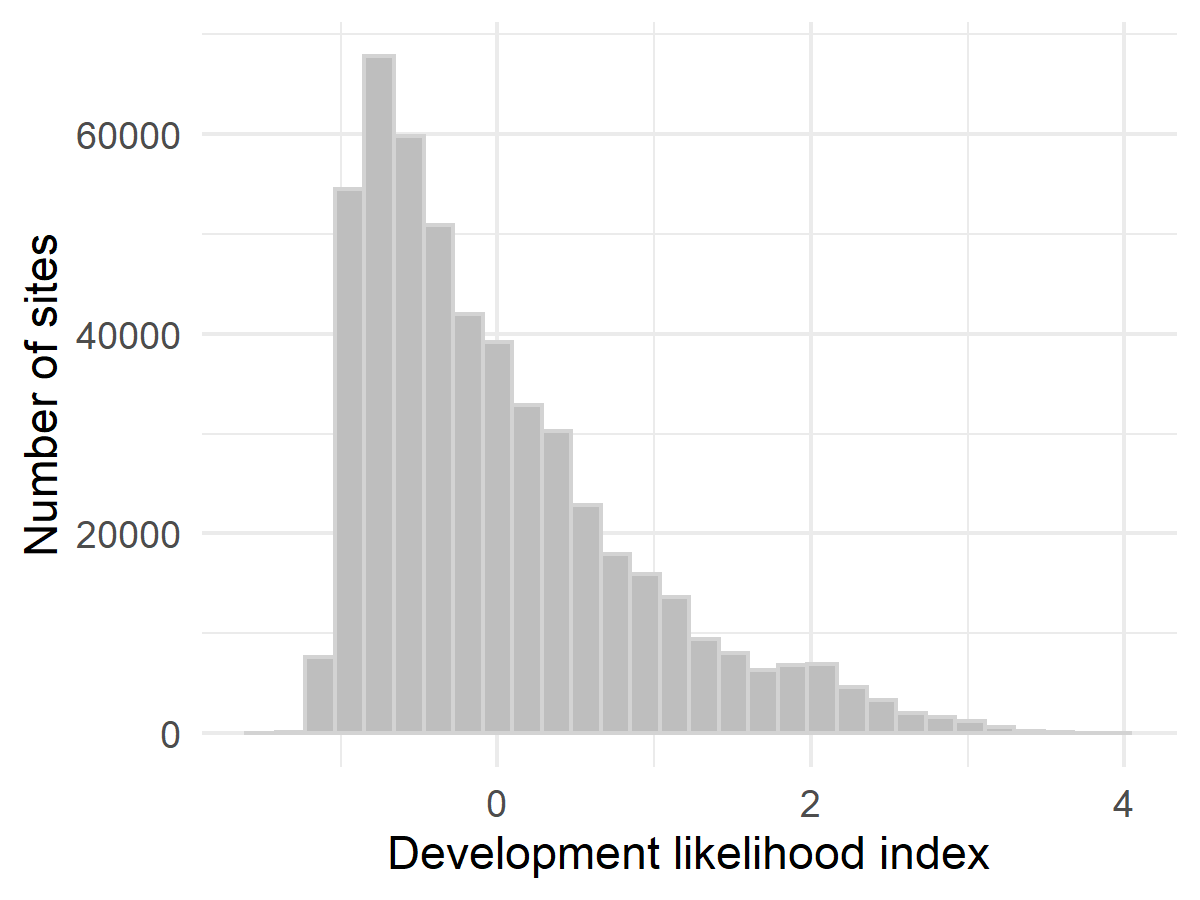
\includegraphics[width=1\linewidth]{04_figures/combined-hist} \caption{Distribution of combined index, weighted according to coefficients from regression predicting the likelihood of a building permit for construction or demolition}\label{fig:combined-hist}
\end{figure}

\begin{figure}
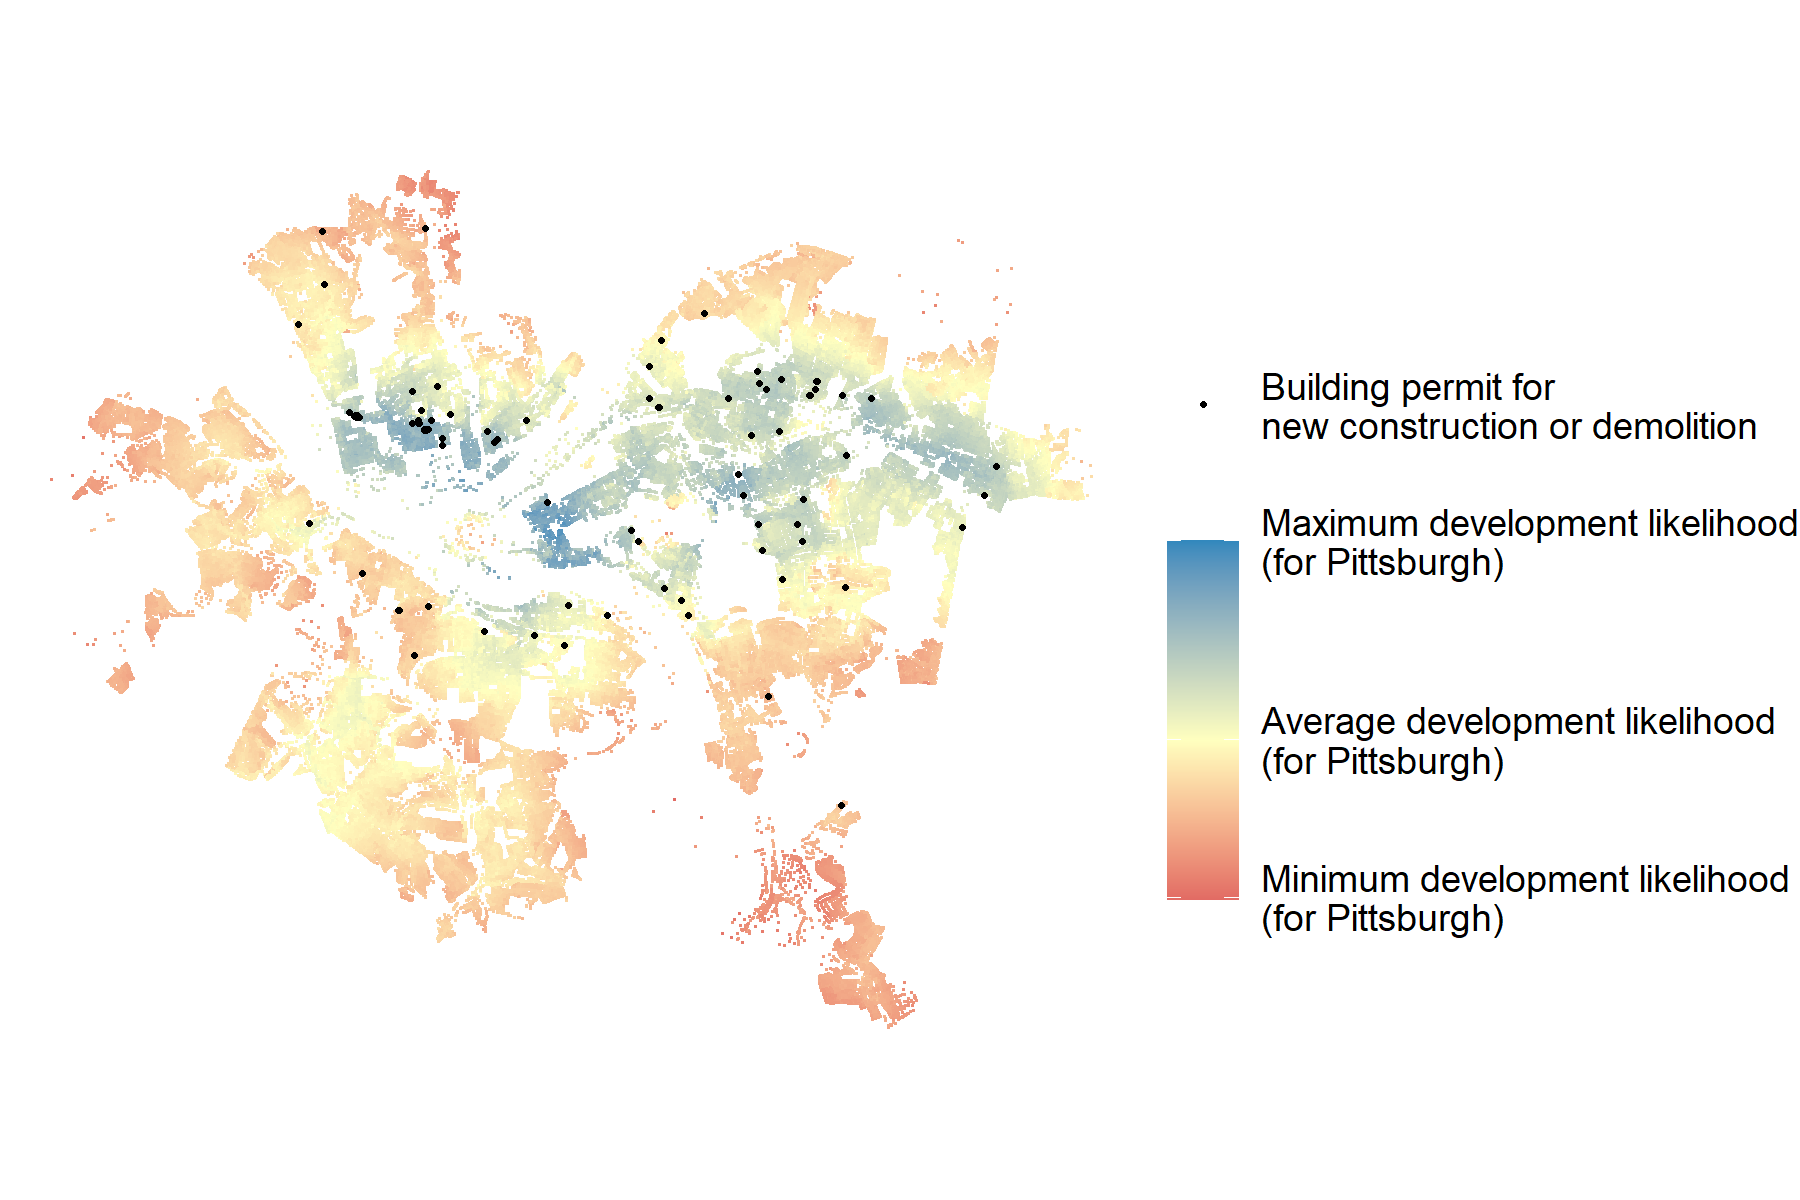
\includegraphics[width=1\linewidth]{04_figures/combined-pitt} \caption{Locations of building permits for new construction and demolition and their estimated likelihood}\label{fig:combined-pitt}
\end{figure}

Figure \ref{fig:combined-map} shows the spatial distribution of the combined index
across the entire study area. It is noteworthy that there is less variation within
the inset area than there is for any of the four indices it comprises. This is because
low scores on one index generally compensate for high scores on another.

\begin{figure}
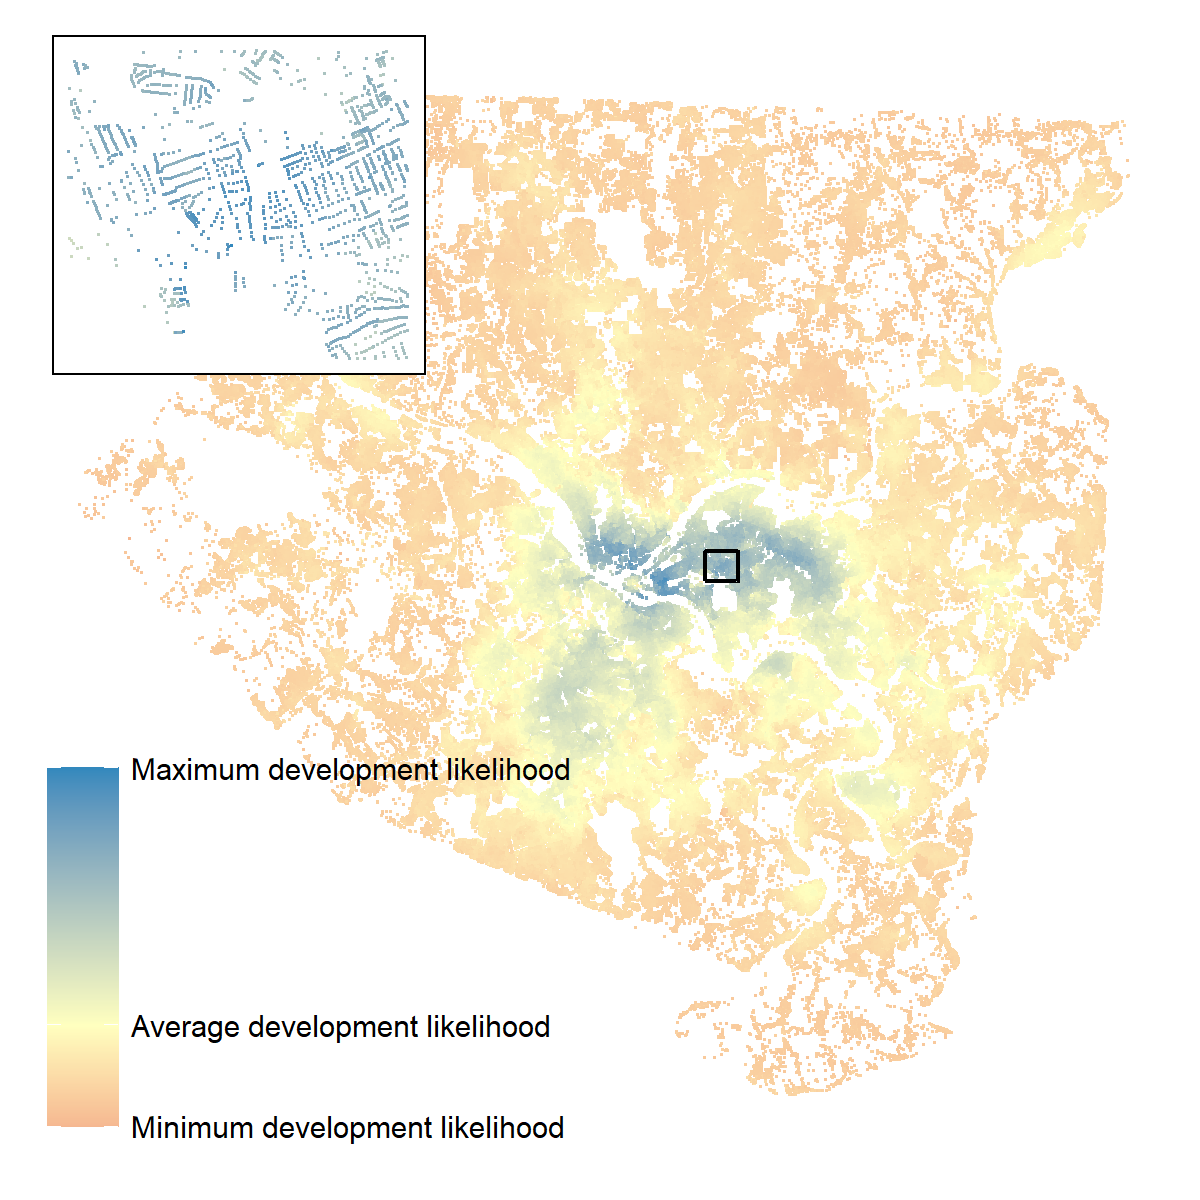
\includegraphics[width=1\linewidth]{04_figures/combined} \caption{Spatial variation in combined index, weighted according to coefficients from regression predicting the likelihood of a building permit for construction or demolition}\label{fig:combined-map}
\end{figure}

\hypertarget{relating-indices-to-values}{%
\chapter{Relating Indices to Values}\label{relating-indices-to-values}}

This chapter will draw connections between the workshop
results and the quantitative analysis results. Elizabeth will write this.

\hypertarget{conclusions-and-future-directions}{%
\chapter{Conclusions and Future Directions}\label{conclusions-and-future-directions}}

Elizabeth to write this chapter.

  \bibliography{book.bib,packages.bib}

\end{document}
